%%%%%%%%%%%%%%%%%%%%%%%%%%%%%%%%%%%%%%%%%%%%%%%%%%%%%%%%%%%%%%%%%%%%%%%%%%
%                          sedFlow User Manual                           %
%%%%%%%%%%%%%%%%%%%%%%%%%%%%%%%%%%%%%%%%%%%%%%%%%%%%%%%%%%%%%%%%%%%%%%%%%%
%
% Copyright (C) 2014 Swiss Federal Research Institute WSL.
% Written by Florian U. M. Heimann
% Published by the Swiss Federal Research Institute WSL
%
% Permission is granted to copy, distribute and/or modify this document
% under the terms of the GNU Free Documentation License, Version 1.3
% published by the Free Software Foundation.
%
% See http://www.gnu.org/licenses for further information.

\documentclass[11pt,a4paper]{article}
\usepackage[utf8]{inputenc}
\usepackage[T1]{fontenc}
\usepackage[english]{babel}

\usepackage{multirow}
\usepackage{chngpage}
\usepackage{multicol}
\usepackage{caption}
\usepackage{float}
\usepackage[pdftex]{graphicx}
\usepackage{epstopdf}

\usepackage{amsmath}
% The following command allows for hfill behaviour within align environment
\makeatletter
\newcommand{\pushright}[1]{\ifmeasuring@#1\else\omit\hfill$\displaystyle#1$\fi\ignorespaces}
\makeatother

\usepackage[numbers]{natbib}

\usepackage{dirtree}
\renewcommand*\DTstyle{\rmfamily}
\renewcommand*\DTstylecomment{\ttfamily}

\newcommand{\DTfolder}[1]{\textbf{\emph{#1}}}
\usepackage[usenames,dvipsnames,svgnames,table]{xcolor}
\newcommand{\DTmainnode}[1]{\textbf{\textcolor{DarkRed}{#1}}}
\newcommand{\DTsimplenode}[1]{\textbf{\textcolor{blue}{#1}}}

\newcommand{\tablefontsize}[0]{\small}

\newcommand{\tbc}[0]{\textcolor{red}{TO BE COMPLETED}}

\usepackage[normalem]{ulem}
\newcommand{\del}[1]{\textcolor{cyan}{\sout{#1}}}
\newcommand{\add}[1]{\textcolor{blue}{\uline{#1}}}

\title{\textbf{\emph{sedFlow}\\User manual}}
\author{Published by the Swiss Federal Research Institute WSL\\Written by Florian U. M. Heimann}
\date{June 2014\\Version 1.00}

\usepackage[pdftex]{hyperref}
\hypersetup{pdfstartview=FitV, pdfcenterwindow=true, bookmarksopen=true, bookmarksopenlevel=2, hidelinks%, pdfstartpage=1
}
\hypersetup{%
	pdftitle={sedFlow - User manual (Version 1.00)},%
	pdfauthor={Published by the Swiss Federal Research Institute WSL and written by Florian U. M. Heimann},%
	pdfsubject={Numeric simulation of fluvial bedload transport in steep mountain streams},%
	pdfkeywords={sedFlow, bedload transport}%
}

% \usepackage{draftwatermark}
% \SetWatermarkScale{7}

\begin{document}

\maketitle
\thispagestyle{empty}
\vfill
The manual is subdivided in two parts: The \emph{Quick start guide} from page~\pageref{QuickStartGuideBegin} to page~\pageref{QuickStartGuideEnd} gives the minimum information to run the model. The \emph{Further specifications} from page~\pageref{FurtherSpecificationsBegin} to page~\pageref{FurtherSpecificationsEnd} complement the short introduction of the \emph{Quick start guide} and gives an in depth description of the different ways to adjust simulation parameters and output formats.

\vspace{\baselineskip}The manual provides an introduction to the use of the model \emph{sedFlow}. For an in depth description of the model please refer to \citet{Heimann++2014a}. Examples of the application of \emph{sedFlow} are given in \citet{Heimann++2014b}.
\vfill
\vfill
Copyright \copyright{} 2014 Swiss Federal Research Institute WSL.

Permission is granted to copy, distribute and/or modify this document under the terms of the GNU Free Documentation License, Version 1.3 published by the Free Software Foundation. See http://www.gnu.org/licenses for further information.

\pagebreak
\setcounter{tocdepth}{3}
\tableofcontents
\vfill
\pagebreak

\part{Quick start guide}
\section{General remarks}\label{GeneralRemarks}
The \label{QuickStartGuideBegin} new model \emph{sedFlow} has been developed to provide an efficient tool for the simulation of bedload transport in mountain streams. The following elements were important for the development of \emph{sedFlow}:
{
\renewcommand{\theenumi}{\roman{enumi}}
\renewcommand{\labelenumi}{(\theenumi)}
\begin{enumerate}
  \item provision of a sediment transport model together with its complete source code open and free of charge
  \item consideration of state of the art approaches for the calculation of bedload transport in steep channels accounting for macro-roughness effects
  \item individual calculation for several grain diameter fractions (fractional transport)
  \item consideration of the effects of adverse slopes in terms of pondages e.g. due to sudden sediment deposition by debris flow inputs
  \item fast calculations for modelling entire catchments, and for automated calculation of many scenarios exploring a range of parameter space
  \item flexibility in model development featuring an object oriented code design
  \item flexibility in model application featuring an easy and straightforward pre- and postprocessing of simulation data.
\end{enumerate}
}
Thus, the model \emph{sedFlow} fills a gap in the range of existing sediment transport models for mountain streams and the mentioned aims have led to the implementation described in the following sections. This implementation represents a current state and may be easily extended and adjusted in the future.

\emph{sedFlow} is a console program without graphical user interface. This format was chosen to enable automated simulation starts within batch or shell scripts and especially to allow for short calculation times. The input files are prepared in other programs. \emph{sedFlow} reads these files and creates output files which are continuously updated in the course of a simulation. To check the progress of a simulation one can take a look at the \emph{ElapsedSeconds} column of any output file. As some programs block files for writing, it is recommended to open copies of an output file as long as the code is still running.

As \emph{sedFlow} is intended for fast simulations (which implies long time steps), executable versions of the code are provided, which will give a warning if the length of the time step falls below a threshold of 1 second or 100 seconds respectively. A version which does not give a warning for short time steps is provided as well.

Most of the simulation data is fed to the model by tabulator delimited text files, which can be created and edited with regular spreadsheet applications such as \emph{Microsoft Excel}. Each such file contains one header line, which defines the number of columns for this file together with the column names. The code selects the data based on the column names. Thus, there is no fixed order for the columns and additional extra columns will be ignored. Empty cells are ignored by the code as well. Within rows containing more elements than the header line, the first elements up to the number of header line entries are used as data entries. Any further entries are ignored. Rows containing less entries than the header line are ignored as well. By this it is easy to include comments in the spreadsheet files.

Most of the simulation parameters are fed to the model by an extensible markup language (xml) input file. For the creation and editing of the input xml file on the \emph{Microsoft Windows} platform the use of the freeware program \emph{Microsoft XML Editor 2007} is recommended. The code will find any information within the xml file based on the position in the node hierarchy and the node name. Additional extra nodes are simply ignored and may be used for commenting.

Any typing errors in the names of the files, columns or nodes will lead to error messages or even worse that the model will ignore the corresponding element without giving a warning at all. Blanks are usually ignored by the code.

In the tables and figures of this manual three question marks (???) indicate a required user input for which no default exists. If such a required input is not given, usually an error message will request it.

\section{Starting the model}\label{StartingTheModel}
The starting point for each simulation is the main input xml file. The location of this file can be given as first argument of the model call e.g. when starting simulations within a script. If the location is not given or the code is started by a simple doubleclick, the model will ask for the location of the file. The location can be given either by an absolute path or by a relative path starting at the location of the model. It is recommended to copy the model into the same folder as the main input xml file and then simply input the name of the xml file.

At the model start the user is requested to hit enter to accept the terms of the license, under which \emph{sedFlow} is distributed. Alternatively, the user may type \emph{acceptLicense} as second argument of the model call, e.g. when starting simulations within a script.

\section{The simulation folder}\label{TheSimulationFolder}
The location of the main input xml file usually defines the simulation folder which always has the same structure (Fig.~\ref{MinimumFolderStructure}).


\begin{figure}[h]
\vspace*{2mm}

\dirtree{%
.1 \DTfolder{myWhateverSimulation}.
.2 myWhateverInput.xml.
.2 \DTfolder{LongitudinalProfile}.
.3 BranchTopology.txt.
.3 BranchXProfile.txt.
.3 \dots{}.
.2 \DTfolder{GrainSizeDistributions}.
.3 myWhateverGrainSizeDistribution.txt.
.3 \dots{}.
.2 \DTfolder{DischargeAndOtherInputs}.
.3 BranchXDischarge.txt.
.3 \dots{}.
.2 \DTfolder{Output}.
.3 \dots{}.
}

\caption{Minimum structure for simulation folder.}
\label{MinimumFolderStructure}
\end{figure}


\section{\emph{BranchTopology.txt}}\label{BranchTopology}
First, the code will go into the folder \emph{LongitudinalProfile} and look for the file \emph{BranchTopology.txt}. Within \emph{sedFlow} the river network is organised in branches. A branch is a section of a river without any tributaries or confluences. Different branches may be connected by confluences. The topology of the river network is defined by the \emph{BranchTopology.txt}. The file contains the two columns \emph{BranchIDs} and \emph{DownstreamBranchIDs} (Tab.~\ref{BranchTopologyTable}), in which the IDs are given as integer numbers. It is required that a branch can only flow into another branch with a higher ID. Examples are given in Figure~\ref{BranchTopologyFigure} and Tables \ref{BranchTopologyRiverNetwork} and \ref{BranchTopologyMainChannelWithStubTributaries}.

\begin{table*}[h]
\caption{Structure of BranchTopology.txt}
\label{BranchTopologyTable}
\vskip4mm
\centering
\begin{tabular}{c|c}
\hline\hline
BranchIDs & DownstreamBranchIDs\\
\hline
??? & ???\\
\hline
$\vdots$ & $\vdots$\\
\hline\hline
\end{tabular}
\end{table*}

\vspace*{2mm}
\begin{center}
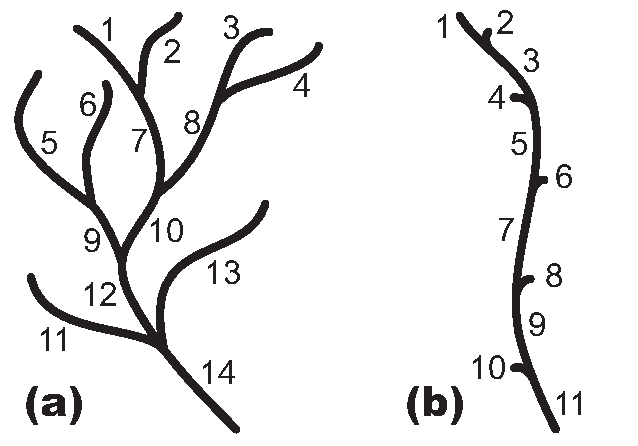
\includegraphics[width=7.5cm]{BranchTopology}
\end{center}
{\captionof{figure}[Examples of potential BranchTopology]{Examples of potential BranchTopology of (a) a river network and (b) a main channel with stub tributaries.} \label{BranchTopologyFigure}}

\begin{multicols}{2}
\begin{table}[H]
\caption{Structure of BranchTopology.txt for river network example of Fig.~\ref{BranchTopologyFigure}a.}
\label{BranchTopologyRiverNetwork}
\vskip4mm
\centering
\begin{tabular}{c|c}
\hline\hline
\multirow{2}{*}{BranchIDs} & Downstream-\\
 & BranchIDs\\
\hline
1 & 7\\
\hline
2 & 7\\
\hline
3 & 8\\
\hline
4 & 8\\
\hline
5 & 9\\
\hline
6 & 9\\
\hline
7 & 10\\
\hline
8 & 10\\
\hline
9 & 12\\
\hline
10 & 12\\
\hline
11 & 14\\
\hline
12 & 14\\
\hline
13 & 14\\
\hline\hline
\end{tabular}
\end{table}

\thispagestyle{empty}
\enlargethispage{20\baselineskip}
\begin{table}[H]
\caption{Structure of BranchTopology.txt for main channel with stub tributaries example of Fig.~\ref{BranchTopologyFigure}b.}
\label{BranchTopologyMainChannelWithStubTributaries}
\vskip4mm
\centering
\begin{tabular}{c|c}
\hline\hline
\multirow{2}{*}{BranchIDs} & Downstream-\\
 & BranchIDs\\
\hline
1 & 3\\
\hline
2 & 3\\
\hline
3 & 5\\
\hline
4 & 5\\
\hline
5 & 7\\
\hline
6 & 7\\
\hline
7 & 9\\
\hline
8 & 9\\
\hline
9 & 11\\
\hline
10 & 11\\
\hline\hline
\end{tabular}
\end{table}
\end{multicols}
\pagebreak

\section{\mbox{\emph{BranchXProfile.txt}}}\label{BranchXProfile}
For each branch defined in the \emph{BranchTopology.txt}, the code will look for a \mbox{\emph{BranchXProfile.txt}} file within the \emph{LongitudinalProfile} folder with \emph{X} substituted by the current branch ID. Within \emph{sedFlow} every branch is discretised into river reaches. Every reach is described by the cross section at its upstream end. Each such cross section is defined by one row in \mbox{\emph{BranchXProfile.txt}}. The file contains at least the following columns (Tab.~\ref{MinimumBranchXProfile}):

\begin{table*}[h]
\caption{Minimum structure of BranchXProfile.txt}
\label{MinimumBranchXProfile}
\vskip4mm
\tablefontsize
\begin{adjustwidth}{-4cm}{-4cm}
\centering
\begin{tabular}{c|c|c|c}
\hline\hline
KilometrageUpstreamDirected & ElevationInM & ChannelWidthInM & StrataGrainSizeDistribution\\
\hline
??? & ??? & ??? & ???\\
\hline
$\vdots$ & $\vdots$ & $\vdots$ & $\vdots$\\
\hline\hline
\end{tabular}
\end{adjustwidth}
\end{table*}

\emph{KilometrageUpstreamDirected} gives an along channel kilometrage which may be e.g. the distance to the river mouth. Within the file, reaches should be sorted from upstream to downstream i.e. the kilometrage values should decrease. It is advisable to define cross sections at roughly equal distances, which should not be smaller than about 50~m. In this context it is important to note that the lowermost cross section of a feeding branch and the uppermost cross section of the recieving branch should \emph{not} be the same. This would define a reach of length zero and lead to kryptic artifacts. Rather, the two profiles should have a distance as described before. In the same way, the lowermost reach of the complete system should also have an adequate length, usually defined by the distance of its cross section to a kilometrage of zero.

\emph{ElevationInM} defines the river bed elevation of the cross section at the upstream end of the reach. Implicitly, this also defines the slope of the reach. When using a kinematic wave routing it is important to make sure that no adverse i.e. negative slopes occur, as they would lead to kryptic artefacts. The slope of the lowermost reach of the system is set equal to the slope of the next upstream reach in front of it.

\emph{ChannelWidthInM} defines the width of the infinitely deep rectangular channel.

\emph{StrataGrainSizeDistribution} defines the file names (without ``.txt'' extension) of the grain size distributions of the alluvium to be used at the start of a simulation. Of course, individual file names may appear repeatedly within this column.

\section{Grain size distributions}\label{GrainSizeDistributions}
For each grain size distribution defined in the \emph{BranchXProfile.txt} files, the code will try to find the corresponding file (Tab.~\ref{GSD}) in the \emph{GrainSizeDistributions} folder. The column \emph{GrainDiameterInCM} usually gives the upper boundaries for the individual grain size fractions. These values need to be sorted in increasing order and need to be identical in all grain size distribution files. The column \emph{RelativeAbundance} gives the relative abundance of the individual fractions (\emph{not} cumulative). The abundances are normalised by the code. Therefore, they do not need to sum up to 1 or 100\%{}.

\begin{table*}[h]
\caption{Structure of grain size distribution spreadsheets}
\label{GSD}
\vskip4mm
\centering
\begin{tabular}{c|c}
\hline\hline
GrainDiameterInCM & RelativeAbundance\\
\hline
??? & ???\\
\hline
$\vdots$ & $\vdots$\\
\hline\hline
\end{tabular}
\end{table*}

\section{\mbox{\emph{BranchXDischarge.txt}}}\label{BranchXDischarge}
The branch topology defines those branches for which no upstream branch is available. For these headwater branches the code tries to find the \mbox{\emph{BranchX}\-\emph{Discharge.txt}} files (Tab.~\ref{Discharge}) within the \emph{DischargeAndOtherInputs} folder with \emph{X} substituted by the corresponding branch ID. The column \emph{ElapsedSeconds} defines the points in time at which a discharge value is given. Of course, these values should increase. The column \emph{DischargeInM3PerS} defines the corresponding discharge values in $\frac{m^3}{s}$. Between the points of this discrete time series, the discharge values are interpolated linearly. Beyond the range of this time series, discharge is constantly set equal to the first or last discharge value respectively. If one wants to feed water (and sediment) at a certain point to the system, it is recommended to introduce a stub branch consisting of just one reach and give a \mbox{\emph{BranchXDischarge.txt}} for it.

\begin{table*}[h]
\caption{Structure of BranchXDischarge.txt}
\label{Discharge}
\vskip4mm
\centering
\begin{tabular}{c|c}
\hline\hline
ElapsedSeconds & DischargeInM3PerS\\
\hline
??? & ???\\
\hline
$\vdots$ & $\vdots$\\
\hline\hline
\end{tabular}
\end{table*}

\section{The main input xml}\label{MinimumMainInputXML}
Most of the simulation data is defined in the spreadsheet files. Most of the simulation parameters will be defined in the main input xml, the location of which already has been discussed in section~\ref{StartingTheModel}. The name of the root node of this file defines the input reader i.e. the way, in which all information is read and interpreted. For this manual the root node name is \mbox{\emph{SEDFLOW\textunderscore{}StandardInput}}. The root node contains at least the two main nodes \emph{overallParameters} and \emph{riverSystemMethods} (Fig.~\ref{MinimumXML}), which will be described in the following. %Examples 
An example 
with potential values %are
is
 given in %Figs.~\ref{MinimumXMLexamplea}~\&~\ref{MinimumXMLexampleb}.
Fig.~\ref{MinimumXMLexamplea}.
For the sake of clarity, the main nodes are printed in dark red in all figures while any other node, which contains child nodes, is printed in blue.

\begin{figure}[h]
\vspace*{2mm}
\dirtree{%
.1 SEDFLOW\_{}StandardInput.
.2 \DTmainnode{overallParameters}.
.3 lowerDiameterBoundaryForFinestFractionInCM\DTcomment{???}.
.2 \DTmainnode{riverSystemMethods}.
.3 \DTsimplenode{sedimentEnergySlopeCalculationMethod}.
.4 realisationType\DTcomment{???}.
.3 \DTsimplenode{bedloadTransportEquations}.
.4 realisationType\DTcomment{???}.
}
\caption{Minimum xml.}
\label{MinimumXML}
\end{figure}

The \emph{overallParameters} collect values of typically single parameters, which are used throughout the complete simulation space and time. It contains at least the node \mbox{\emph{lowerDiameterBoundaryForFinestFractionInCM}}, which defines the lower boundary for the finest grain size fraction. Make sure that its value is smaller than the smallest diameter of the grain size distribution files (section~\ref{GrainSizeDistributions}).

The \emph{riverSystemMethods} typically collect the procedures and algorithms which are used in the course of a simulation. The names of the nodes specify the job, which is to be fulfilled by the corresponding method. The child nodes specify the way in which the method fulfills its job. Typically, there is always one child node called \emph{realisation} to select the general algorithm of the current method. Depending on the realisation there may be other child nodes defining further parameters, which are specific for the current realisation. Different realisations and their various parameters are described in section~\ref{Realisations}. The \emph{riverSystemMethods} contain at least the nodes \emph{sedimentEnergySlopeCalculationMethod} and \emph{bedloadTransportEquations}. The node \emph{sedimentEnergySlopeCalculationMethod} is mainly used to determine whether or not the energy slope for the determination of bedload transport capacity should be reduced in order to account for flow resistance partitioning. The node \emph{bedloadTransportEquations} defines the way, in which the bedload transport capacity is estimated. The recommended combination %s
of realisations is %are
\emph{WithFlowResistancePartitioning} and \emph{RickenmannBedloadCapacityBasedOnTheta} (Fig.~\ref{MinimumXMLexamplea}).% or \emph{NoFlowResistancePartitioning} and \emph{SchneiderEtAlBedloadCapacity} (Fig.~\ref{MinimumXMLexampleb}). (The \emph{SchneiderEtAlBedloadCapacity} method has been derived using bedslopes and based on data from steep mountain catchments. Therefore, it should not be combined with \emph{WithFlowResistancePartitioning}, as it would underestimate transport capacity in this combination.)


\begin{figure}[h]
\vspace*{2mm}
\dirtree{%
.1 SEDFLOW\_{}StandardInput.
.2 \DTmainnode{overallParameters}.
.3 lowerDiameterBoundaryForFinestFractionInCM\DTcomment{0.2}.
.2 \DTmainnode{riverSystemMethods}.
.3 \DTsimplenode{sedimentEnergySlopeCalculationMethod}.
.4 realisationType\DTcomment{WithFlowResistancePartitioning}.
.3 \DTsimplenode{bedloadTransportEquations}.
.4 realisationType\DTcomment{RickenmannBedloadCapacityBasedOnTheta}.
}
\caption{Minimum xml with recommended values.}% (combination a).}
\label{MinimumXMLexamplea}
\end{figure}

% \begin{figure}[h]
% \vspace*{2mm}
% \dirtree{%
% .1 SEDFLOW\_{}StandardInput.
% .2 \DTmainnode{overallParameters}.
% .3 lowerDiameterBoundaryForFinestFractionInCM\DTcomment{0.2}.
% .2 \DTmainnode{riverSystemMethods}.
% .3 \DTsimplenode{sedimentEnergySlopeCalculationMethod}.
% .4 realisationType\DTcomment{NoFlowResistancePartitioning}.
% .3 \DTsimplenode{bedloadTransportEquations}.
% .4 realisationType\DTcomment{SchneiderEtAlBedloadCapacity}.
% }
% \caption{Minimum xml with recommended values (combination b).}
% \label{MinimumXMLexampleb}
% \end{figure}

Please consider the cautionary notes given in section~\ref{WaterFlowRoutingRealisations} related to the water flow routing method \emph{UniformDischarge}, which is used by default in the setup of Figure~\ref{MinimumXML}\label{QuickStartGuideEnd}.

\pagebreak
\part{Further specifications}
\label{FurtherSpecificationsBegin}

The \emph{Quick start guide} on the previous pages described the minimum amount of information which is needed to run a simulation. In such a case, many simulation parameters are set to their default values. The user can override these default values simply by adding further files to the simulation folder or further columns to the spreadsheet files or further nodes to the input xml file. (It is important to note that complete columns need to be given. Even if only one value differs from the default, the complete column needs to be input with the defaults given explicitly and the single other value. If default values are not given and the corresponding rows have therefore less entries than the header line, these rows will be ignored completely.)

\begin{figure}[h]
\vspace*{2mm}

\dirtree{%
.1 \DTfolder{myWhateverSimulation}.
.2 myWhateverInput.xml.
.2 \DTfolder{LongitudinalProfile}.
.3 BranchTopology.txt.
.3 BranchXProfile.txt.
.3 \dots{}.
.3 Sills.txt.
.2 \DTfolder{GrainSizeDistributions}.
.3 myWhateverGrainSizeDistribution.txt.
.3 \dots{}.
.2 \DTfolder{DischargeAndOtherInputs}.
.3 BranchXDischarge.txt.
.3 \dots{}.
.3 SedimentInputs.txt.
.3 myWhateverSedigraph.txt.
.3 \dots{}.
.3 InstantaneousSedimentInputs.txt.
.2 \DTfolder{Output}.
.3 \dots{}.
}

\caption{Complete structure for simulation folder.}
\label{CompleteFolderStructure}
\end{figure}


The complete structure for the simulation folder including all possible input files is displayed in Figure~\ref{CompleteFolderStructure}. The complete structure of the \emph{BranchXProfile.txt} spreadsheet files including all possible columns is described in section~\ref{CompleteBranchXProfile} and summarised in the Tables~\ref{CompleteBranchXProfile1}~\&{}~\ref{CompleteBranchXProfile2}. Predefined sediment inputs may be included in a simulation by additional files in the \emph{DischargeAndOtherInputs} folder as described in section~\ref{SedimentInput}. The influence of sills may be considered in a simulation by including an additional file in the \emph{LongitudinalProfile} folder as described in section~\ref{Sills}. The complete structure for the input xml file is described in the section~\ref{CompleteXML} and an example of the complete xml structure is summarised in the Figures~\ref{OverallParametersXML}~to~\ref{OutputMethodsAdditionalXML}.

\section[Complete BranchXProfile.txt]{Complete structure for BranchXProfile.txt}
\label{CompleteBranchXProfile}

The complete structure of \emph{BranchXProfile.txt} is summarised in the Tables~\ref{CompleteBranchXProfile1}~\&{}~\ref{CompleteBranchXProfile2}. The columns \emph{KilometrageUpstreamDirected}, \emph{ElevationInM}, \emph{ChannelWidthInM} and \emph{StrataGrainSizeDistribution} have been described in section~\ref{BranchXProfile}.

The \emph{AlluviumThicknessInM} defines the amount of erodible material in a reach. If this column is not given the model will set its values to 4000.0 by default.

As described in section~\ref{BranchXProfile}, the \emph{StrataGrainSizeDistribution} defines the grain size distributions of the alluvium to be used at the start of a simulation. It is possible to define an initial grain size distribution for the surface or active layer which may differ from the rest of the alluvium. To do so, one adds the column \emph{SurfaceLayerGrainSizeDistribution} which defines the surface layer grain size distribution file names (without the .txt extension). If this column is not given, the code will use the file names of \emph{StrataGrainSizeDistribution} for the definition of the initial \emph{SurfaceLayerGrainSizeDistribution}.

\emph{BedrockRoughnessEquivalentRepresentativeGrainDiameterInCM} defines the flow resistance and hiding properties of a reach, when the river runs over bedrock and there is no grain size distribution left to define the properties of the reach. For example, if a flow resistance relation is based on the 84\textsuperscript{th} percentile grain diameter $D_{84}$, the values in this column will be used as $D_{84}$ for this flow resistance relation. It is advisable to select values close to the measured grain diameters in this area. If the alluvium cover gets thin, the local grain sizes will tendentially approach the value of the bedrock roughness. If the column \emph{BedrockRoughnessEquivalentRepresentativeGrainDiameterInCM} is not given, the code will use the $D_{84}$ of the grain size distributions given in the \emph{SurfaceLayerGrainSizeDistribution}.

\begin{table*}[h]
\caption{Complete structure of BranchXProfile.txt (part 1)}
\label{CompleteBranchXProfile1}
\vskip4mm
\tablefontsize
\begin{adjustwidth}{-4cm}{-4cm}
\centering
\begin{tabular}{c|c|c|c|c}
\hline\hline
KilometrageUpstreamDirected & ElevationInM & ChannelWidthInM & AlluviumThicknessInM & $\cdots$\\
\hline
??? & ??? & ??? & 4000.0 & $\cdots$\\
\hline
$\vdots$ & $\vdots$ & $\vdots$ & $\vdots$ & $\vdots$\\
\hline\hline
\end{tabular}
\end{adjustwidth}
\end{table*}


\begin{table*}[h]
\caption{Complete structure of BranchXProfile.txt (part 2) including default values}
\label{CompleteBranchXProfile2}
\vskip4mm
\tablefontsize
\begin{adjustwidth}{-4cm}{-4cm}
\centering
\begin{tabular}{c|c|c|c}
\hline\hline
\multirow{2}{*}{$\cdots$} & Strata- & SurfaceLayer- & BedrockRoughnessEquivalent-\\
 & GrainSizeDistribution & GrainSizeDistribution & RepresentativeGrainDiameterInCM\\
\hline
\multirow{2}{*}{$\cdots$} & \multirow{2}{*}{???} & file name of & $D_{84}$ of\\
 & & StrataGrainSizeDistribution & SurfaceLayerGrainSizeDistribution\\
\hline
$\vdots$ & $\vdots$ & $\vdots$ & $\vdots$\\
\hline\hline
\end{tabular}
\end{adjustwidth}
\end{table*}

\section{Sediment input}\label{SedimentInput}
\subsection{Transport capacity input}\label{TransportCapacityInput}
The transport capacity input is the default way to feed sediment to the system. At the start of a simulation, the reaches at the upstream ends of the simulated river system are copied to create virtual margin reaches just outside the boundaries of the simulated system. The elevation, grain size distribution and alluvium thickness of these margin cells are kept constant for the complete simulation. Within these margin cells, bedload transport capacity is calculated corresponding to the grain size distribution of its active layer, its width \&{} slope and the current discharge. The calculated bedload tranport capacity is then fed to the simulated river system. Therefore it is recommended to define the most upstream reaches in a way to be representative for the transport system of the headwaters, which are not simulated. If no sediment is to be fed to the system, it is recommended to set the alluvium thickness to zero in the corresponding topmost reach. (A value close to zero will not do the job, as alluvium thickness is not eroded in the virtual margin reaches.)

\subsection{Sedigraph input}\label{SedigraphInput}
In order to input sediment independent of the discharge, one can define sedigraphs. For this, the optional file \emph{SedimentInputs.txt} is put into the \emph{DischargeAndOtherInputs} folder. The file (Tabs.~\ref{SedimentInputs1}~\&{}~\ref{SedimentInputs2}) contains at least the columns \emph{BranchIDs}, \emph{KilometrageUpstreamDirected}, \emph{GrainSizeDistribution} and \emph{SedimentInputTimeSeries}.

\begin{table*}[h]
\caption{Structure of SedimentInputs.txt (part 1)}
\label{SedimentInputs1}
\vskip4mm
\tablefontsize
\centering
\begin{tabular}{c|c|c|c}
\hline\hline
BranchIDs & KilometrageUpstreamDirected & GrainSizeDistribution & $\cdots$\\
\hline
??? & ??? & ??? & $\cdots$\\
\hline
$\vdots$ & $\vdots$ & $\vdots$ & $\vdots$\\
\hline\hline
\end{tabular}
\end{table*}


\begin{table*}[h]
\caption{Structure of SedimentInputs.txt (part 2) including default values}
\label{SedimentInputs2}
\vskip4mm
\tablefontsize
\begin{adjustwidth}{-4cm}{-4cm}
\centering
\begin{tabular}{c|c|c|c}
\hline\hline
\multirow{2}{*}{$\cdots$} & \multirow{2}{*}{SedimentInputTimeSeries} & ReplacingRegularDepositionRate- & \multirow{2}{*}{InputIncludingPoreVolume}\\
 & & InsteadOfAddingToIt & \\
\hline
$\cdots$ & ??? & false & true\\
\hline
$\vdots$ & $\vdots$ & $\vdots$ & $\vdots$\\
\hline\hline
\end{tabular}
\end{adjustwidth}
\end{table*}

The \emph{BranchIDs} and \emph{KilometrageUpstreamDirected} define the crosssection, at which the sediment is fed to the system. So if sediment enters the river channel between two crosssections, one would simply input the branch ID and kilometrage of the more downstream profile. If the code cannot match branch ID and kilometrage to an existing profile, it will simply ignore the corresponding row in the \emph{SedimentInputs.txt}. The \emph{GrainSizeDistribution} defines the file name (without the .txt extension) for the grain size distribution of the sediment input. The code will look for the specified files in the \emph{GrainSizeDistributions} folder. Please note that the grain size distribution of the sediment input stays the same for the complete simulation. It will \emph{not} become coarser at high input rates and it will \emph{not} become finer at low input rates. To mimic such behaviour one may either use the transport capacity input as described in section~\ref{TransportCapacityInput} or one may feed multiple sediment inputs with different grain size distributions to the same reach. The \emph{SedimentInputTimeSeries} define the file names of the different time series of sediment flux fed to the simulated channel. The code will look for these files in the \emph{DischargeAndOtherInputs} folder. The structure of these time series files (Tab.~\ref{Sedigraph}) and the way, in which they are read by the code, correspond to the discharge time series as described in section~\ref{BranchXDischarge}.

\begin{table*}[h]
\caption{Structure of sedigraph spreadsheets}
\label{Sedigraph}
\vskip4mm
\centering
\begin{tabular}{c|c}
\hline\hline
ElapsedSeconds & SedimentInputInM3PerS\\
\hline
??? & ???\\
\hline
$\vdots$ & $\vdots$\\
\hline\hline
\end{tabular}
\end{table*}

Please note that the model reads the sediment input rate at the beginning of a time step and keeps this value for the complete time step. This means that the temporal discretisation of the sediment input time series should not be finer than the average time step of the simulation. Any input event which is shorter than the average time step will not be captured properly by this input mechanism.

The sedigraph input is usually added to the material coming from upstream. To modify this, one adds the optional column \emph{ReplacingRegularDepositionRateInsteadOfAddingToIt}. One of the rare applications of this option is the simulation of a retention basin with a defined downstream sediment yield (which may be zero as well). If the column \emph{ReplacingRegularDepositionRateInsteadOfAddingToIt} is not included in the \emph{SedimentInputs.txt}, its values are set to \emph{false} by default.

The sediment inputs are usually considered to include pore volume. To modify this, one adds the optional column \emph{InputIncludingPoreVolume}. If the column is not given, its values are set to \emph{true} by default.

\subsection{Instantaneous sediment pulse input}\label{InstantaneousSedimentPulseInput}
As mentioned before, sediment input events, which are shorter than the average time step, cannot be represented by sedigraph inputs as described in section~\ref{SedigraphInput}. To account for such events one adds the file \emph{InstantaneousSedimentInputs.txt} to the \emph{DischargeAndOtherInputs} folder. This file contains the columns \emph{BranchIDs}, \emph{KilometrageUpstreamDirected}, \emph{GrainSizeDistribution}, \emph{InputVolumesInM3}, \emph{ElapsedSeconds} and \emph{InputIncludingPoreVolume}, in which \emph{InputIncludingPoreVolume} can be left out to set all its values to \emph{true}. All columns except \emph{InputVolumesInM3} and \emph{ElapsedSeconds} are treated in the way which is described in section~\ref{SedigraphInput}. The \emph{InputVolumesInM3} define the volume of sediment which is to be fed to a certain reach and the \emph{ElapsedSeconds} define the point in time in which this shall happen.

\begin{table*}[h]
\caption{Structure of InstantaneousSedimentInputs.txt (part 1)}
\label{InstantaneousSedimentInputs1}
\vskip4mm
\tablefontsize
\centering
\begin{tabular}{c|c|c|c}
\hline\hline
BranchIDs & KilometrageUpstreamDirected & GrainSizeDistribution & $\cdots$\\
\hline
??? & ??? & ??? & $\cdots$\\
\hline
$\vdots$ & $\vdots$ & $\vdots$ & $\vdots$\\
\hline\hline
\end{tabular}
\end{table*}


\begin{table*}[h]
\caption{Structure of InstantaneousSedimentInputs.txt (part 2) including default values}
\label{InstantaneousSedimentInputs2}
\vskip4mm
\tablefontsize
\centering
\begin{tabular}{c|c|c|c}
\hline\hline
$\cdots$ & InputVolumesInM3 & ElapsedSeconds & InputIncludingPoreVolume\\
\hline
$\cdots$ & ??? & ??? & true\\
\hline
$\vdots$ & $\vdots$ & $\vdots$ & $\vdots$\\
\hline\hline
\end{tabular}
\end{table*}

\section{Sills}\label{Sills}
The large scale effects of sills i.e. the dissipation of energy can be considered within \emph{sedFlow} simulations. A sill is represented by the fixed elevation of the top edge of the sill and the variable elevation of the river bed just downstream of the sill (disregarding local effects such as the stilling pool). The slope upstream of the sill is calculated using the elevation difference between the next upstream cross section and the maximum of the fixed sill top edge and the variable bed just downstream of the sill. The maximum function allows for the consideration of the burial of sills. The slope downstream of the sill is calculated using the elevation difference between the variable bed just downstream of the sill and the next downstream cross section. To simulate a series of sills with distances between them, which are smaller than the ideal distance of cross sections, it is recommended to substitute the series of sills by one single sill with an elevation drop equal to the sum of elevation drops of the complete series of sills. As only the large scale effects of sills are considered, the results will be the same and with one single sill it is possible to keep the ideal distance of cross sections. All outputs for a cross section with a sill refer to the variable bed just downstream of the sill. The evolution at the top edge of the sill is not displayed as it can be trivially derived.

To introduce sills one adds the optional \emph{Sills.txt} to the folder \emph{LongitudinalProfile}. The columns \emph{BranchID} and \emph{KilometrageUpstreamDirected} define the reach at which a sill should be introduced. If no existing reach can be found to match the branch ID and kilometrage, the corresponding sill entry is ignored. The \emph{SillTopEdgeElevationInM} gives the absolute elevation of the top edge of the sill. It should equal the elevation of the corresponding reach plus the elevation drop of the sill. Alternatively the column \emph{SillDropHeightInM} can be given. In this case, the elevation of the sill top edge is calculated as the sum of the drop height and the elevation of the corresponding reach. If both columns are given, the values from the \emph{SillTopEdgeElevationInM} are used. Please note that the top edge elevation is fixed, while the drop height may change in the course of a simulation as the crosssection at the sill may experience erosion or accumulation of sediment. The sill hydraulics are calculated according to the so called Poleni equation:

\begin{equation}
Q = \frac{2}{3} \cdot \mu \cdot \sqrt{2 \cdot g} \cdot w \cdot h^{\frac{3}{2}}
\end{equation}

In this, $Q$ is discharge; $g$ is gravity acceleration; $w$ is flow width and $h$ is hydraulic head at the sill. The weir coefficient $\mu$ is defined by the column \emph{PoleniFactor}. If this column is not given, its values are set to $\sqrt{\frac{1}{3}}$ by default.

The way in which the bed elevation upstream of a sill is updated, may be defined by node \emph{upstreamOfSillsWedgeShapedInsteadOfParallelUpdate} in the main input xml. For details see section~\ref{RiverSystemMethods}.

\begin{table*}[h]
\caption{Structure of Sills.txt including default values}
\label{SillsFile}
\vskip4mm
\begin{adjustwidth}{-4cm}{-4cm}
\centering
\begin{tabular}{c|c|c|c}
\hline\hline
\multirow{2}{*}{BranchIDs} & \multirow{2}{*}{KilometrageUpstreamDirected} & SillTopEdgeElevationInM & \multirow{2}{*}{PoleniFactor}\\
 & & \textbf{or} SillDropHeightInM & \\
\hline
??? & ??? & ??? & $\sqrt{\frac{1}{3}}$\\
\hline
$\vdots$ & $\vdots$ & $\vdots$ & $\vdots$\\
\hline\hline
\end{tabular}
\end{adjustwidth}
\end{table*}

\section{Complete structure of the main input xml file}\label{CompleteXML}
The structure of the main input xml as described in section~\ref{MinimumMainInputXML} represents only a minimum to run a \emph{sedFlow} simulation. The following sections describe all potential nodes and their default values which are inserted, if a node is not given. The summarising illustrations (Figs.~\ref{OverallParametersXML}~to~\ref{OutputMethodsAdditionalXML}) just give one possible example of a complete input xml structure including all default values.

\subsection{\emph{overallParameters}}\label{OverallParameters}

\begin{figure}[p]
\vspace*{2mm}
\dirtree{%
.1 SEDFLOW\_{}StandardInput.
.2 \DTmainnode{overallParameters}.
.3 inputUpperBoundaryInsteadOfMeanGrainDiameter\DTcomment{true}.
.3 lowerDiameterBoundaryForFinestFractionInCM\DTcomment{???}.
.3 useArithmeticMeanInsteadOfGeometricMeanForFractionGrainDiameters\DTcomment{false}.
.3 densityWater\DTcomment{1000.0}.
.3 densitySediment\DTcomment{2650.0}.
.3 poreVolumeFraction\DTcomment{0.3}.
.3 gravityAcceleration\DTcomment{9.80665}.
.3 angleOfReposeInDegree\DTcomment{36.0}.
.3 elapsedSeconds\DTcomment{Min of first discharge file}.
.3 finishSeconds\DTcomment{Max of first discharge file}.
.3 courantFriedrichsLewyNumber\DTcomment{0.9}.
.3 timeStepThresholdForTerminatingSimulation\DTcomment{0.0000000001}.
.3 timeStepFactor\DTcomment{1.0}.
.3 kilometrageOfSimulationOutlet\DTcomment{0.0}.
.3 thicknessInputsIncludingPoreVolume\DTcomment{true}.
.2 \DTmainnode{riverSystemMethods}.
.3 \dots{}.
.2 \DTmainnode{outputMethods}.
.3 \dots{}.
}
\caption{overallParameters including default values.}
\label{OverallParametersXML}
\end{figure}

\emph{inputUpperBoundaryInsteadOfMeanGrainDiameter} is used to switch the way in which the \emph{GrainDiameterInCM} column of the grain size distribution files is interpreted. If it is true (default value), the diameters are interpreted as upper fraction boundaries and the representative fraction diameter is calculated as the mean of the boundaries. If it is false, the diameters given in the grain size distribution files are directly used as representative fraction diameters.

The \emph{lowerDiameterBoundaryForFinestFractionInCM}, which has been already described in section~\ref{MinimumMainInputXML}, is only needed if \emph{inputUpperBoundaryInsteadOfMeanGrainDiameter} is \emph{true}.

If \emph{inputUpperBoundaryInsteadOfMeanGrainDiameter} is \emph{true}, the \emph{useArithmeticMeanInsteadOfGeometricMeanForFractionGrainDiameters} is used to switch between the geometric (default) and arithmetic mean for the representative fraction diameter.

The \emph{densityWater} and \emph{densitySediment} define the liquid and solid densities in $\frac{kg}{m^3}$ with their default values of 1000.0 and 2650.0 respectively.

The \emph{poreVolumeFraction} defines the volumetric portion of pores and fine (suspension load) sediment with its default value of 0.3.

The \emph{gravityAcceleration} given in $\frac{m}{s^2}$ has a default value of 9.80665.

The \emph{angleOfReposeInDegree} has a default value of 36.0.
%\textcolor{red}{Sollte man hier noch was schreiben?}

The \emph{elapsedSeconds} and \emph{finishSeconds} define the start and end of the simulation. By default they are set to the minimum and maximum of the \emph{ElapsedSeconds} column of the \emph{BranchXDischarge.txt}, with X equal to the smallest used branch ID.

The \emph{courantFriedrichsLewyNumber} is used to determine numerically stable time step lengths. It represents the maximum potential value for the ratio $\frac{v \cdot \Delta{}t}{\Delta{}x}$, in which $v$ is velocity and $\Delta{}x$ \&{} $\Delta{}t$ are spatial \&{} temporal discretisation. The default value for the Courant-Friedrichs-Lewy number is 0.9.

As \emph{sedFlow} is intended for fast simulations with long time steps, the simulation will stop whenever the time step length drops below the \emph{timeStepThresholdForTerminatingSimulation}, as this points to some problems in the current simulation. The default value for this threshold is 0.0000000001.

The \emph{timeStepFactor} may be used to modify the time step lengths, which the model determines based on its criteria for numeric stability. Its default value is 1.0 and it is not recommended to use the option of changing this value.

The length of the lowermost river reach is calculated as the difference between its kilometrage from the \emph{BranchXProfile.txt} and the \emph{kilometrageOfSimulationOutlet}. By default, the simulations start at a kilometrage of 0.0.

The switch \emph{thicknessInputsIncludingPoreVolume} is used to define whether or not thickness inputs such as e.g. the erodible alluvium thickness are considered to include the pore volume. The default value of this node is \emph{true}.

\subsection{\emph{riverSystemMethods}}\label{RiverSystemMethods}

The switch \emph{upstreamOfSillsWedgeShapedInsteadOfParallelUpdate} determines the way, in which the bed elevation upstream of a sill (section~\ref{Sills}) is updated. If the switch is \emph{false}, the model assumes that erosion and deposition are equally distributed within the completete reach, which is also assumed in any other reach not affected by a sill. If the switch is \emph{true}, the model assumes that erosion and deposition are distributed in a wedge-shaped way within the reach. This will cause the bed elevation upstream of a sill to adjust twice as fast as in reaches not affected by sills. If the node is not given, its value is set to \emph{false} by default.

The nodes \emph{bedSlopeCalculationMethod}, \emph{waterEnergySlopeCalculationMethod} and \emph{sedimentEnergySlopeCalculationMethod} define the way in which the bed slope and the energy slope for the hydraulic and sediment transport capacity calculations is determined. Different realisations are described in section~\ref{GradientCalculationMethodRealisations}. However it is not recommended to change the default values of \emph{bedSlopeCalculationMethod} and \emph{waterEnergySlopeCalculationMethod}. If these nodes are not given, their realisation types are set to the \emph{SimpleDownstreamTwoCellGradient} of \emph{elevation} (section~\ref{SimpleDownstreamTwoCellGradient}) and the \emph{ReturnBedslope} (section~\ref{ReturnBedslopeAndReturnWaterEnergyslope}) by default. For \emph{sedimentEnergySlopeCalculationMethod} the realisations \emph{WithFlowResistancePartitioning} or \emph{NoFlowResistancePartitioning} (both section~\ref{GradientCalculationMethodRealisations}) are recommended.

The \emph{flowResistance} node defines the way in which average flow velocity and wetted cross section area are determined for a given discharge. Different realisations are described in section~\ref{FlowResistanceRealisations}. Please note that for the \emph{ImlicitKinematicWave} flow routing (section~\ref{ImplicitKinematicWave}) only the \emph{FixedPowerLawFlowResistance} flow resistance (section~\ref{FixedPowerLawFlowResistance}) can be used. However, the \emph{VariablePowerLawFlowResistance} (section~\ref{VariablePowerLawFlowResistance}) is assumed to better represent the processes in steep mountain channels. If the \emph{flowResistance} node is not given, its realisation type is set to \emph{FixedPowerLawFlowResistance} (if the \emph{waterFlowRouting} realisation is \emph{ImplicitKinematicWave}) or to \emph{VariablePowerLawFlowResistance} (in any other case) by default.

The node \emph{bedloadVelocityCalculationMethod} defines the way to estimate grain velocities, which are only needed and used to check for the bedload flux the Courant-Friedrichs-Lewy criterion of numeric stability. Different realisations are described in section~\ref{BedloadVelocityCalculationMethodRealisations}. If the node \emph{bedloadVelocityCalculationMethod} is not given, its realisation is set to \emph{VelocityAsTranpsportRatePerUnitCrossSectionalArea} (section~\ref{VelocityAsTranpsportRatePerUnitCrossSectionalArea}) by default.

The node \emph{tauCalculationMethod} defines the way to estimate the bed shear stress. Different realisations are described in section~\ref{TauCalculationMethodRealisations}. If the node is not given, its realisation is set to \emph{EnergyslopeTau} (section~\ref{TauCalculationMethodRealisations}) by default.

The node \emph{activeWidthCalculationMethod} defines the way to estimate the width in which sediment transport takes place. At the moment \emph{SetActiveWidthEqualFlowWidth} is the only realisation for this node. Alternative methods may be implemented in future versions of \emph{sedFlow}.

The \emph{waterFlowRouting} node defines the way in which water is transferred through the channel system and how the \emph{flowResistance} relation is applied to calculate flow depths and velocities. Different realisations are described in section~\ref{WaterFlowRoutingRealisations}. The \emph{ExplicitKinematicWave} (section~\ref{ExplicitKinematicWave}) and \emph{ImplicitKinematicWave} (section~\ref{ImplicitKinematicWave}) depend on positive bed slopes. The \emph{ImplicitKinematicWave} (section~\ref{ImplicitKinematicWave}) further depends on the \emph{FixedPowerLawFlowResistance} flow resistance (section~\ref{FixedPowerLawFlowResistance}), the approximation of the hydraulic radius by flow depth (section~\ref{FlowResistanceRealisations}) and on an infinitely deep rectangular channel, which is given anyway. The \emph{UniformDischarge} (section~\ref{UniformDischarge}) has no dependencies and replaces the discharge routing approach by a uniform discharge approach.

The node \emph{bedloadTransportEquations} defines the way in which the bedload transport capacity is estimated. Different realisations are described in section~\ref{BedloadTransportEquationsRealisations}. Fractional transport as well as representative single grain size approaches can be selected. However, single grain size approaches do not imply an increase in calculation speed, as the model framework is optimised for fractional approaches.

The node \emph{strataSorting} defines the interaction between the surface active layer and the subsurface alluvium. Different realisations are described in section~\ref{StrataSortingRealisations}. If the node \emph{strataSorting} is not given, its realisation is set to \emph{TwoLayerWithShearStressBasedUpdate} (section~\ref{TwoLayerWithShearStressBasedUpdate}) by default.

The optional node \emph{additionalMethods} may be added to include further methods, which are not covered by the aforementioned \emph{riverSystemMethods} nodes. Up to now the only \emph{additionalMethods} are concerned with the effects of gravel abrasion (section~\ref{additionalMethodsWithSternbergAbrasion}).

\pagebreak
\dirtree{%
.1 SEDFLOW\_{}StandardInput.
.2 \DTmainnode{overallParameters}.
.3 \dots{}.
.2 \DTmainnode{riverSystemMethods}.
.3 upstreamOfSillsWedgeShapedInsteadOfParallelUpdate\DTcomment{false}.
.3 \DTsimplenode{bedSlopeCalculationMethod}.
.4 realisationType\DTcomment{SimpleDownstreamTwoCellGradient}.
.4 propertyOfInterest\DTcomment{elevation}.
.3 \DTsimplenode{waterEnergySlopeCalculationMethod}.
.4 realisationType\DTcomment{ReturnBedslope}.
.4 minimumSlope\DTcomment{-inf}.
.3 \DTsimplenode{sedimentEnergySlopeCalculationMethod}.
.4 realisationType\DTcomment{WithFlowResistancePartitioning}.
.4 stressPartitioningExponent\DTcomment{1.5}.
.4 calculationBasedOnqInsteadOfh\DTcomment{false}.
.4 maximumFroudeNumber\DTcomment{value from flowResistance}.
.4 minimumInputSlope\DTcomment{???}.
.4 ensureMinimumInputSlope\DTcomment{if minimumInputSlope node exists}.
.3 \DTsimplenode{flowResistance}.
.4 startingValueForIteration\DTcomment{0.4}.
.4 accuracyForTerminatingIteration\DTcomment{0.001}.
.4 maximumNumberOfIterations\DTcomment{400}.
.4 typeOfNumericRootFinder\DTcomment{RiddersMethod}.
.4 useApproximationsForHydraulicRadius\DTcomment{If waterFlowRouting == ImplicitKinematicWave}.
.4 maximumFroudeNumber\DTcomment{4.0}.
.4 minimumHydraulicSlope\DTcomment{0.0004}.
.4 realisationType\DTcomment{VariablePowerLawFlowResistance}.
.3 \DTsimplenode{bedloadVelocityCalculationMethod}.
.4 realisationType\DTcomment{VelocityAsTransportRatePerUnitCrossSectionalArea}.
.4 \DTsimplenode{estimateThicknessOfMovingSedimentLayer}.
.5 realisationType\DTcomment{ConstantThicknessOfMovingSedimentLayer}.
.5 constantThickness\DTcomment{0.7}.
.3 \DTsimplenode{tauCalculationMethod}.
.4 realisationType\DTcomment{EnergyslopeTau}.
.4 correctionForBedloadWeightAtSteepSlopes\DTcomment{true}.
.3 \DTsimplenode{activeWidthCalculationMethod}.
.4 realisationType\DTcomment{SetActiveWidthEqualFlowWidth}.
.3 \dots{}.
.2 \DTmainnode{outputMethods}.
.3 \dots{}.
}
{\captionof{figure}{riverSystemMethods part 1 including default values.}\label{RiverSystemMethods1XML}}

\pagebreak
\thispagestyle{empty}
\enlargethispage{5\baselineskip}
\dirtree{%
.1 SEDFLOW\_{}StandardInput.
.2 \DTmainnode{overallParameters}.
.3 \dots{}.
.2 \DTmainnode{riverSystemMethods}.
.3 \dots{}.
.3 \DTsimplenode{waterFlowRouting}.
.4 realisationType\DTcomment{UniformDischarge}.
.4 maximumTimeStep\DTcomment{900}.
.3 \DTsimplenode{bedloadTransportEquations}.
.4 maximumFractionOfActiveLayerToBeEroded\DTcomment{0.9}.
.4 preventZeroOrNegativeBedSlopes\DTcomment{if waterFlowRouting == some KinematicWave}.
.4 maximumRelativeTwoCellBedSlopeChange\DTcomment{0.9}.
.4 realisationType\DTcomment{RickenmannBedloadCapacityBasedOnTheta}.
.4 useOnePointOneAsExponentForFroudeNumber\DTcomment{false}.
.4 simplifiedEquation\DTcomment{true}.
.4 thetaCriticalBasedOnConstantSred\DTcomment{false}.
.4 \DTsimplenode{thresholdCalculationMethod}.
.5 realisationType\DTcomment{LambEtAlCriticalTheta}.
.5 minimumCriticalDimensionlessShearStress\DTcomment{0.03}.
.5 correctionForBedloadWeightAtSteepCounterSlopes\DTcomment{true}.
.4 \DTsimplenode{hidingFactorsCalculationMethod}.
.5 realisationType\DTcomment{PowerLawHidingFunction}.
.5 referenceDiameterPercentile\DTcomment{50.0}.
.5 exponent\DTcomment{-0.8}.
.3 \DTsimplenode{strataSorting}.
.4 realisationType\DTcomment{TwoLayerWithShearStressBasedUpdate}.
.4 dynamicLayerThickness\DTcomment{false}.
.4 useInitialGrainSizesForConstantLayerThickness\DTcomment{true}.
.4 layerThicknessFactor\DTcomment{1.75}.
.4 referenceGrainSizePercentile\DTcomment{84.0}.
.4 layerThickness\DTcomment{only needed if neither dynamicLayerThickness nor useInitialGrainSizesForConstantLayerThickness}.
.4 dynamicBreakUpConditions\DTcomment{false}.
.4 usePredefinedBreakUpConditions\DTcomment{false}.
.4 referenceMedianDiameter\DTcomment{only needed if usePredefinedBreakUpConditions}.
.4 thetaCriticalForActiveLayer\DTcomment{only needed if usePredefinedBreakUpConditions}.
.4 thetaCriticalForSublayer\DTcomment{only needed if usePredefinedBreakUpConditions}.
.4 \DTsimplenode{thresholdCalculationMethod}\DTcomment{method from bedloadTransportEquations or default displayed there}.
.3 \DTsimplenode{additionalMethods}\DTcomment{optional}.
.2 \DTmainnode{outputMethods}.
.3 \dots{}.
}
{\captionof{figure}{riverSystemMethods part 2 including default values.}\label{RiverSystemMethods2XML}}

\subsection{\emph{outputMethods}}\label{OutputMethods}
\subsubsection{Standard and regular outputs}\label{StandardAndRegularOutputs}

\paragraph{General remarks}
Within \emph{sedFlow} the format of the output files can be defined globally by the standard output properties. Alternatively single output files can be defined individually by the regular output nodes. In both cases the nodes are the same. For the standard output properties the term ``Standard'' is added to the node name and the nodes are direct child nodes of the \emph{OutputMethods} node. For individual files the node \emph{regularOutput} or the nodes \emph{regularOutputX} may be added to the \emph{OutputMethods}. In this, \emph{X} is replaced by an integer number starting at 1 and going up to the desired number of files. If there is a break in the sequence of \emph{X} values, the following nodes will be ignored. The nodes for the formatting of output files are described in the following:

\paragraph{Output file formatting}
The node \emph{forVisualInterpretation} is used to switch between the usual output format for numeric postprocessing using other programmes and a version for a more visual and by-hand postprocessing workflow. The usual format has a single line header and no additional formatting symbols. The \emph{forVisualInterpretation} version has a header which consists of several rows and has extra columns with formatting symbols, which separate the individual properties and reaches. This format is useful, when different properties for only a few reaches are written to a single file, which shall be evaluated in a by-hand postprocessing.

The \emph{precisionForOutput} defines the precision for the output of floating point numbers. Please note that floating point numbers are output in scientific format convention. For long simulation times, make sure that the output precision is sufficient to discriminate the different \emph{ElapsedSeconds} values.

By \emph{outputTimeStepLength} an additional column with the current time step length in seconds may be added to the output file.

By \emph{outputInitialValues} an output row with the values at the start of the simulation is added. This makes sense for some state properties like elevation or grain diameter percentiles. For other properties like e.g. the transport rate, which are calculated in the course of a simulation, dummy values will be printed.

As described in section~\ref{TransportCapacityInput}, the code internally creates virtual margin reaches at the upstream ends and at the downstream end of the simulated system. These margin reaches are used to feed inputs to the system and to recieve the outflux at the downstream end. The \emph{printUpstreamMargins} and the \emph{printDownstreamMargin} switches may be used to add these virtual margin reaches to the output file. This option is mainly intended for debugging.

\paragraph{Output timing}
The \emph{explicitTimesForOutput} may contain a series of child nodes, which define certain points in time (expressed as elapsed seconds), at which an output row shall be written. The names of the child nodes are ignored.

The \emph{outputInterval} defines the interval in seconds, at which output rows shall be written.

The \emph{writeLineEachTimeStep} may be used to enforce the output of every simulated time step. This option is intended for debugging and not recommended for daily use.

In \emph{sedFlow} it is possible to use a secondary output interval, which is applied, when some property like e.g. discharge exceeds a certain threshold. This may be used to e.g. increase output frequency during floods. For the standard, the secondary interval is used, when one of the four nodes \emph{referenceCellIDStandard}, \emph{referencePropertyStandard}, \emph{thresholdToBeExceededStandard} or \emph{secondaryOutputIntervalStandard} is given. For individual outputs the secondary interval is used, when the node \emph{SecondaryOutputInterval} is given, which contains the four mentioned nodes. The node \emph{referenceProperty} defines the property, for which it is checked whether it exceeds some threshold. The node \emph{referenceCellID} defines the ID of the reach, at which it is checked whether the reference property exceeds a threshold. The node \emph{thresholdToBeExceeded} defines the threshold, which needs to be exceeded for the application of the secondary output interval. Finally, the \emph{secondaryOutputInterval} defines the output interval, which is applied whenever the threshold is exceeded.

\paragraph{Selecting output reaches and properties}
The node \emph{reachIDsForOutput} is used to select the reaches, for which output should be written to files. This node contains child nodes with the possible names \emph{reachID} and \emph{branchID}. The branch IDs are used as defined in the \emph{branchTopology.txt}. The reach IDs are used as defined in the \emph{reachIDExplanations.txt}, which is written to the \emph{Output} folder by the model. If the node \emph{reachIDsForOutput} is not given, the model will produce outputs for all reaches by default.

The node \emph{regularRiverReachPropertiesForOutput} defines for which properties the values shall be written to the output files. The node contains child nodes, the names of which define the output properties. With the standard outputs, the code will create one file for each property, if the switch \emph{createStandardOutputs} is \emph{true} (default). For the individual outputs all properties will be written into one file. Potential values for the \emph{regularRiverReachPropertiesForOutput} are the following:

\begin{multicols}{3}
\begin{itemize}
	\item \emph{elevation}
	\item \emph{length}
	\item \emph{sillOccurence}
	\item \emph{sillTopEdgeElevation}
	\item \emph{discharge}
	\item \emph{flowVelocity}
	\item \emph{maximumWaterdepth}
	\item \emph{waterLevel}
	\item \emph{hydraulicHead}
	\item \emph{kineticComponent-}\emph{OfHydraulicHead}
	\item \emph{bedShearStress}
	\item \emph{activeWidth}
	\item \emph{strataPerUnit-}\emph{BedSurface}
	\item \emph{strataPerUnit-}\emph{BedSurface-}\emph{IncludingPoreVolume}
	\item \emph{alluviumThickness-}\emph{IncludingPoreVolume}
	\item \emph{bedrockElevation}
	\item \emph{bedslope}
	\item \emph{waterEnergyslope}
	\item \emph{sedimentEnergyslope}
	\item \emph{unreduced-}\emph{SedimentEnergyslope}
	\item \emph{waterVolumeChangeRate}
	\item \emph{waterVolumeChange}
\end{itemize}
\end{multicols}
\vspace{3ex}
\begin{multicols}{2}
\begin{itemize}
	\item \emph{activeLayerPerUnitBedSurface}
	\item \emph{activeLayerPerUnitBedSurface-}\emph{IncludingPoreVolume}
	\item \emph{activeLayerPerUnitBedSurface-}\emph{OverallVolume}
	\item \emph{activeLayerPerUnitBedSurface-}\emph{OverallVolumeIncludingPoreVolume}
	\item \emph{activeLayerPerUnitBedSurface-}\emph{MedianGrainDiameter}
	\item \emph{activeLayerPerUnitBedSurface-}\emph{ArithmeticMeanGrainDiameter}
	\item \emph{activeLayerPerUnitBedSurface-}\emph{GeometricMeanGrainDiameter}
	\item \emph{activeLayerPerUnitBedSurfaceD20}
	\item \emph{activeLayerPerUnitBedSurfaceD30}
	\item \emph{activeLayerPerUnitBedSurfaceD50}
	\item \emph{activeLayerPerUnitBedSurfaceD84}
	\item \emph{activeLayerPerUnitBedSurfaceD90}
\end{itemize}
\end{multicols}
\vspace{3ex}
\begin{multicols}{2}
\begin{itemize}
	\item \emph{erosionRate}
	\item \emph{erosionRateIncludingPoreVolume}
	\item \emph{erosionRateOverallVolume}
	\item \emph{erosionRateOverallVolume-}\emph{IncludingPoreVolume}
	\item \emph{erosionRateMedianGrainDiameter}
	\item \emph{erosionRateArithmeticMean-}\emph{GrainDiameter}
	\item \emph{erosionRateGeometricMean-}\emph{GrainDiameter}
	\item \emph{erosionRateD20}
	\item \emph{erosionRateD30}
	\item \emph{erosionRateD50}
	\item \emph{erosionRateD84}
	\item \emph{erosionRateD90}
\end{itemize}
\end{multicols}
\vspace{3ex}
\begin{multicols}{2}
\begin{itemize}
	\item \emph{depositionRate}
	\item \emph{depositionRateIncludingPoreVolume}
	\item \emph{depositionRateOverallVolume}
	\item \emph{depositionRateOverallVolume-}\emph{IncludingPoreVolume}
	\item \emph{depositionRateMedianGrainDiameter}
	\item \emph{depositionRateArithmeticMean-}\emph{GrainDiameter}
	\item \emph{depositionRateGeometricMean-}\emph{GrainDiameter}
	\item \emph{depositionRateD20}
	\item \emph{depositionRateD30}
	\item \emph{depositionRateD50}
	\item \emph{depositionRateD84}
	\item \emph{depositionRateD90}
\end{itemize}
\end{multicols}
\vspace{3ex}
\begin{multicols}{2}
\begin{itemize}
	\item \emph{erosion}
	\item \emph{erosionIncludingPoreVolume}
	\item \emph{erosionOverallVolume}
	\item \emph{erosionOverallVolume-}\\ \emph{IncludingPoreVolume}
	\item \emph{erosionMedianGrainDiameter}
	\item \emph{erosionArithmeticMean-}\emph{GrainDiameter}
	\item \emph{erosionGeometricMean-}\emph{GrainDiameter}
	\item \emph{erosionD20}
	\item \emph{erosionD30}
	\item \emph{erosionD50}
	\item \emph{erosionD84}
	\item \emph{erosionD90}
\end{itemize}
\end{multicols}
\vspace{3ex}
\begin{multicols}{2}
\begin{itemize}
	\item \emph{deposition}
	\item \emph{depositionIncludingPoreVolume}
	\item \emph{depositionOverallVolume}
	\item \emph{depositionOverallVolume-}\emph{IncludingPoreVolume}
	\item \emph{depositionMedianGrainDiameter}
	\item \emph{depositionArithmeticMean-}\emph{GrainDiameter}
	\item \emph{depositionGeometricMean-}\emph{GrainDiameter}
	\item \emph{depositionD20}
	\item \emph{depositionD30}
	\item \emph{depositionD50}
	\item \emph{depositionD84}
	\item \emph{depositionD90}
\end{itemize}
\end{multicols}
\vspace{3ex}
\begin{multicols}{2}
\begin{itemize}
	\item \emph{erosionPerUnitBedSurface}
	\item \emph{erosionPerUnitBedSurface-}\emph{IncludingPoreVolume}
	\item \emph{erosionPerUnitBedSurface-}\emph{OverallVolume}
	\item \emph{erosionPerUnitBedSurface-}\emph{OverallVolumeIncludingPoreVolume}
	\item \emph{erosionPerUnitBedSurface-}\emph{MedianGrainDiameter}
	\item \emph{erosionPerUnitBedSurface-}\emph{ArithmeticMeanGrainDiameter}
	\item \emph{erosionPerUnitBedSurface-}\emph{GeometricMeanGrainDiameter}
	\item \emph{erosionPerUnitBedSurfaceD20}
	\item \emph{erosionPerUnitBedSurfaceD30}
	\item \emph{erosionPerUnitBedSurfaceD50}
	\item \emph{erosionPerUnitBedSurfaceD84}
	\item \emph{erosionPerUnitBedSurfaceD90}
\end{itemize}
\end{multicols}
\vspace{3ex}
\begin{multicols}{2}
\begin{itemize}
	\item \emph{depositionPerUnitBedSurface}
	\item \emph{depositionPerUnitBedSurface-}\emph{IncludingPoreVolume}
	\item \emph{depositionPerUnitBedSurface-}\emph{OverallVolume}
	\item \emph{depositionPerUnitBedSurface-}\emph{OverallVolumeIncludingPoreVolume}
	\item \emph{depositionPerUnitBedSurface-}\emph{MedianGrainDiameter}
	\item \emph{depositionPerUnitBedSurface-}\emph{ArithmeticMeanGrainDiameter}
	\item \emph{depositionPerUnitBedSurface-}\emph{GeometricMeanGrainDiameter}
	\item \emph{depositionPerUnitBedSurfaceD20}
	\item \emph{depositionPerUnitBedSurfaceD30}
	\item \emph{depositionPerUnitBedSurfaceD50}
	\item \emph{depositionPerUnitBedSurfaceD84}
	\item \emph{depositionPerUnitBedSurfaceD90}
\end{itemize}
\end{multicols}

The \emph{erosionRate} properties display the potential local transport capacity in $\frac{m^3}{s}$ not considering supply limitations. The \emph{erosion} properties display the actual local transport in $m^3$ considering supply limitations. For the actual local transport rate, the \emph{erosion} properties have to be divided by the current time step length. The \emph{erosionPerUnitBedSurface} properties display the \emph{erosion} properties normalised to a column of $1 m^2$ base area. The \emph{depositionRate} and \emph{deposition} properties are usually equal to the \emph{erosionRate} and \emph{erosion} properties of the upstream reach. If there are several upstream neighbours, the \emph{depositionRate} and \emph{deposition} properties display the sum of the upstream values. Local \emph{depositionRate} or \emph{deposition} may differ from the upstream  \emph{erosionRate} or \emph{erosion}, if the effects of gravel abrasion (section~\ref{additionalMethodsWithSternbergAbrasion}) are simulated.

\paragraph{Output file naming}
If an output file contains only one property, the file will have the name of this property by default. If a file contains several properties, it will be named regularOutput or regularOutputX by default corresponding to the name of its node. These default names may be overridden by the node \emph{name}. Please note that if a file name (default or user defined) is used several times, several output routines will write to the same file creating cryptic artefacts.

\paragraph{\emph{outputAccumulatedBedloadTransport}}
Within the regular and standard output files, all values represent a snapshot of the property at a specified point in time. That is, the values are \emph{not} integrated over an output interval or the complete simulation time. However, the important descriptive variable of the accumulated bedload transport is defined as the temporal integral of the local transport rates. Therefore, the \emph{regularOutputX} nodes are complemented by the \emph{outputAccumulatedBedloadTransportX} nodes, which may be used to output the temporal integral of the bedload transport rates. (Within the \emph{regularRiverReachPropertiesForOutputStandard} the pseudo property \emph{accumulatedBedloadTransport} may be used to create an output file corresponding to \emph{outputAccumulatedBedloadTransportX}.) The \emph{outputAccumulatedBedloadTransportX} contains the following child nodes, which are used as described for \emph{regularOutputX}: \emph{explicitTimesForOutput}, \emph{outputInterval}, \emph{precisionForOutput}, \emph{reachIDsForOutput} and \emph{writeLineEachTimeStep}. The switch \emph{outputIncludingPoreVolume} defines whether the displayed volumes shall include pore volume or just represent the solid material. The default for \emph{outputIncludingPoreVolume} is \emph{true}, as any volumetric data recorded in the field commonly includes the pore volume as well. By default, the \emph{outputAccumulatedBedloadTransport} will create a file with the overall transported volumes. The switch \emph{outputDetailedFractional} is used to create an additional file, in which the transported volumes are specified for each grain size fraction separately. To discriminate these two types of files, the suffixes ``ABT-OverallVolume'' or ``ABT-DetailedFractional'' are appended to the (by default empty) file name, which is specified by the node \emph{name}.

\subsubsection{\emph{backupXML}}\label{backupXML}
For very long simulations, it is possible to create backups of the current state of a running simulation. To do so, one adds the node \emph{backupXML} to the \emph{outputMethods}. The child nodes \emph{explicitTimesForOutput}, \emph{outputInterval} and \emph{precisionForOutput} are used as described for standard and regular outputs in section~\ref{StandardAndRegularOutputs}. By default, any new backup will replace the previous one. To change this, one sets \emph{overwriteFiles} to \emph{false}. In this case an ID will be appended to the file name. The number of digits of this ID can be changed using the \emph{numberOfFileIDDigits} node. For multiple backups it may be worth to redirect these files from the standard \emph{Output} folder, where they are stored by default, to some other location, which is given in the node \emph{alternativePathForXMLBackupOutputs}. To restart a simulation from a backup, one simply starts \emph{sedFlow} and imports the backup file instead of the normal main input xml (section~\ref{MinimumMainInputXML}). In general, it is not recommended to create backup files, as this considerably slows down a simulation.

\subsubsection{\emph{outputSimulationSetup}}\label{outputSimulationSetup}
By default the model creates an easy to read summary of the current simulation setup. To supress this output, one sets the node \emph{notOutputSimulationSetup} to \emph{true}. The format of the output can be defined within the \emph{outputSimulationSetup} node. The child node \emph{precisionForOutput} is used as described for standard and regular outputs in section~\ref{StandardAndRegularOutputs}. The selection and order of the displayed setup properties is defined in the \emph{setupPropertiesForOutput}. The default values are \emph{CalcBedloadCapacity}, \emph{FlowResistance}, \emph{CalcGradient} and \emph{StrataSorting}. Other potential values are \emph{CalcTau} and \emph{CalcActiveWidth}. The file name can be changed using the node \emph{name}. The \emph{simulationID} and \emph{simulationName} can be used to include any user defined text to the output file. The switch \emph{printStartingTime} defines whether the starting time of the simulation shall be included to the file and the switch \emph{printModelVersion} selects whether the compilation date of the used model binary shall be included to the file as well. By default the value of both switches is \emph{true}.

\pagebreak
\thispagestyle{empty}
\enlargethispage{2\baselineskip}
\dirtree{%
.1 SEDFLOW\_{}StandardInput.
.2 \DTmainnode{overallParameters}.
.3 \dots{}.
.2 \DTmainnode{riverSystemMethods}.
.3 \dots{}.
.2 \DTmainnode{outputMethods}.
.3 createStandardOutputs\DTcomment{true}.
.3 forVisualInterpretationStandard\DTcomment{false}.
.3 explicitTimesForOutputStandard\DTcomment{empty}.
.3 outputIntervalStandard\DTcomment{3600.0}.
.3 precisionForOutputStandard\DTcomment{4}.
.3 writeLineEachTimeStepStandard\DTcomment{false}.
.3 outputTimeStepLengthStandard\DTcomment{false}.
.3 outputInitialValuesStandard\DTcomment{true}.
.3 printUpstreamMarginsStandard\DTcomment{false}.
.3 printDownstreamMarginStandard\DTcomment{false}.
.3 \DTsimplenode{reachIDsForOutputStandard}\DTcomment{all reach IDs}.
.3 useSecondaryOutputInterval\DTcomment{if one of the following four nodes exists}.
.3 referenceCellIDStandard\DTcomment{???}.
.3 referencePropertyStandard\DTcomment{???}.
.3 thresholdToBeExceededStandard\DTcomment{???}.
.3 secondaryOutputIntervalStandard\DTcomment{???}.
.3 \DTsimplenode{regularRiverReachPropertiesForOutputStandard}.
.4 elevation.
.4 activeLayerPerUnitBedSurfaceD50.
.4 activeLayerPerUnitBedSurfaceD84.
.4 bedslope.
.4 maximumWaterdepth.
.4 accumulatedBedloadTransport.
.3 notOutputSimulationSetup\DTcomment{false}.
.3 \DTsimplenode{outputSimulationSetup}.
.4 name\DTcomment{SimulationSetup.txt}.
.4 precisionForOutput\DTcomment{standard value}.
.4 simulationID\DTcomment{empty}.
.4 simulationName\DTcomment{empty}.
.4 printStartingTime\DTcomment{true}.
.4 printModelVersion\DTcomment{true}.
.4 \DTsimplenode{setupPropertiesForOutput}.
.5 CalcBedloadCapacity.
.5 FlowResistance.
.5 CalcGradient.
.5 StrataSorting.
.3 \dots{}.
}
{\captionof{figure}{outputMethods standard including default values.}\label{OutputMethodsStandardXML}}

\pagebreak
\dirtree{%
.1 SEDFLOW\_{}StandardInput.
.2 \DTmainnode{overallParameters}.
.3 \dots{}.
.2 \DTmainnode{riverSystemMethods}.
.3 \dots{}.
.2 \DTmainnode{outputMethods}.
.3 \dots{}.
.3 \DTsimplenode{regularOutputX}.
.4 forVisualInterpretation\DTcomment{standard value}.
.4 \DTsimplenode{regularRiverReachPropertiesForOutput}.
.5 \dots{}.
.4 name\DTcomment{name of PropertyForOutput or regularOutputX}.
.4 explicitTimesForOutput\DTcomment{standard value}.
.4 outputInterval\DTcomment{standard value}.
.4 precisionForOutput\DTcomment{standard value}.
.4 \DTsimplenode{reachIDsForOutput}\DTcomment{standard value}.
.4 writeLineEachTimeStep\DTcomment{standard value}.
.4 outputTimeStepLength\DTcomment{standard value}.
.4 outputInitialValues\DTcomment{standard value}.
.4 printUpstreamMargins\DTcomment{standard value}.
.4 printDownstreamMargin\DTcomment{standard value}.
.4 \DTsimplenode{SecondaryOutputInterval}.
.5 referenceCellID\DTcomment{standard value}.
.5 referenceProperty\DTcomment{standard value}.
.5 thresholdToBeExceeded\DTcomment{standard value}.
.5 secondaryOutputInterval\DTcomment{standard value}.
.3 \DTsimplenode{outputAccumulatedBedloadTransportX}.
.4 name\DTcomment{empty}.
.4 explicitTimesForOutput\DTcomment{standard value}.
.4 outputInterval\DTcomment{standard value}.
.4 precisionForOutput\DTcomment{standard value}.
.4 reachIDsForOutput\DTcomment{standard value}.
.4 writeLineEachTimeStep\DTcomment{standard value}.
.4 outputIncludingPoreVolume\DTcomment{true}.
.4 outputDetailedFractional\DTcomment{false}.
.3 \DTsimplenode{backupXML}.
.4 alternativePathForXMLBackupOutputs\DTcomment{empty}.
.4 explicitTimesForOutput\DTcomment{standard value}.
.4 outputInterval\DTcomment{standard value}.
.4 precisionForOutput\DTcomment{standard value}.
.4 overwriteFiles\DTcomment{true}.
.4 numberOfFileIDDigits\DTcomment{4}.
}
{\captionof{figure}{outputMethods regular including default values.}\label{OutputMethodsAdditionalXML}}

\section{Realisations}\label{Realisations}
%\textcolor{red}{Sollte hier noch eine Einleitung geschrieben werden? Wenn ja, welche?}
\subsection{\emph{flowResistance} realisations}\label{FlowResistanceRealisations}
\label{FirstRealisationsSection}
\emph{flowResistance} methods are intended to determine the $\sqrt{\frac{8}{f}}$ in the following equation:
\begin{equation}
\sqrt{\frac{8}{f}} = \frac{v}{\sqrt{g \cdot r_h \cdot S_f}}
\end{equation}
In this, $f$ is the Darcy-Weisbach friction factor; $v$ is flow velocity; $g$ is gravitational acceleration; $r_h$ is hydraulic radius and $S_f$ is friction slope.

To deal with numeric issues all \emph{flowResistance} realisations (Fig.~\ref{flowResistanceXML}) have the following optional nodes: \emph{startingValueForIteration}, \emph{accuracyForTerminatingIteration}, \emph{maximumNumberOfIterations} and \emph{typeOfNumericRootFinder}. Potential values for \emph{typeOfNumericRootFinder} are \emph{BisectionMethod}, \emph{SecantMethod}, \emph{FalsePositionMethod} and \emph{RiddersMethod}, among which the \emph{RiddersMethod} is recommended.

The switch \emph{useApproximationsForHydraulicRadius} defines whether the hydraulic radius should be approximated by flow depth. By default, it  is \emph{true}, if \emph{ImplicitKinematicWave} is selected as \emph{waterFlowRouting}, and \emph{false} in any other case.

If \emph{UniformDischarge} is selected as \emph{waterFlowRouting}, the code will ensure that the Froude number will not exceed a maximum and that the hydraulic slope will not fall below a minimum. The respective values are defined in the nodes \emph{maximumFroudeNumber} and \emph{minimumHydraulicSlope}.

\begin{figure}[H]
\vspace*{2mm}
\dirtree{%
.1 \DTsimplenode{flowResistance}.
.2 startingValueForIteration\DTcomment{0.4}.
.2 accuracyForTerminatingIteration\DTcomment{0.001}.
.2 maximumNumberOfIterations\DTcomment{400}.
.2 typeOfNumericRootFinder\DTcomment{RiddersMethod}.
.2 useApproximationsForHydraulicRadius\DTcomment{If waterFlowRouting == ImplicitKinematicWave}.
.2 maximumFroudeNumber\DTcomment{4.0}.
.2 minimumHydraulicSlope\DTcomment{0.0004}.
.2 \dots{}.
}
\caption{flowResistance including default values.}
\label{flowResistanceXML}
\end{figure}

\subsubsection{\emph{FixedPowerLawFlowResistance}}\label{FixedPowerLawFlowResistance}
The \emph{FixedPowerLawFlowResistance} (Fig.~\ref{FixedPowerLawFlowResistanceXML}) has four optional nodes, which can be derived from the following equation:
\begin{equation}
\sqrt{\frac{8}{f}} = j \cdot \left( \frac{r_h}{k \cdot D_x} \right)^l
\end{equation}
The value of $j$ is defined by the node \emph{factor} with its default value of $6.5$. The value of $k$ is defined by the node \emph{grainsFactor} with its default value of $1.0$. $D_x$ is the x'th percentile grain diameter with the value of $x$ defined by the node \emph{grainsPercentile} with its default value of $84.0$. The value of $l$ is defined by the node \emph{exponent} with its default value of $0.166666667$.

\begin{figure}[H]
\vspace*{2mm}
\dirtree{%
.1 \DTsimplenode{flowResistance}.
.2 \dots{}.
.2 realisationType\DTcomment{FixedPowerLawFlowResistance}.
.2 factor\DTcomment{6.5}.
.2 grainsFactor\DTcomment{1.0}.
.2 grainsPercentile\DTcomment{84.0}.
.2 exponent\DTcomment{0.166666667}.
}
\caption{FixedPowerLawFlowResistance including default values.}
\label{FixedPowerLawFlowResistanceXML}
\end{figure}

If one uses the default value of $\sim{}\frac{1}{6}$ for the \emph{exponent} $l$, this method corresponds to a Manning-Strickler flow resistance relation with:
\begin{equation}
k_{st} = \frac{1}{n} = \frac{j \cdot \sqrt{g}}{\left(k \cdot D_x\right)^{\frac{1}{6}}},
\end{equation}
\noindent{}in which $k_{st}$ is the Strickler roughness coefficient and $n$ is the Manning roughness coefficient.

If one uses all default values, this method corresponds to a Manning-Strickler flow resistance relation with:
\begin{equation}
k_{st} = \frac{1}{n} = \frac{6.5 \cdot \sqrt{g}}{D_{84}^{\frac{1}{6}}}
\end{equation}

\subsubsection{\emph{VariablePowerLawFlowResistance}}\label{VariablePowerLawFlowResistance}
The \emph{VariablePowerLawFlowResistance} (Fig.~\ref{VariablePowerLawFlowResistanceXML}) implements the following equation from \citet{Ferguson2007} with the parameter values by \citet{Rickenmann+2011} and has no specific additional nodes.
\begin{equation}
\sqrt{\frac{8}{f}} = \frac{6.5 \cdot 2.5 \cdot \frac{r_h}{D_{84}}}{\sqrt{6.5^2 + 2.5^2 \cdot \left( \frac{r_h}{D_{84}} \right)^\frac{5}{3}}}
\end{equation}

\begin{figure}[H]
\vspace*{2mm}
\dirtree{%
.1 \DTsimplenode{flowResistance}.
.2 \dots{}.
.2 realisationType\DTcomment{VariablePowerLawFlowResistance}.
}
\caption{VariablePowerLawFlowResistance.}
\label{VariablePowerLawFlowResistanceXML}
\end{figure}

\subsection{\emph{waterFlowRouting} realisations}\label{WaterFlowRoutingRealisations}
It has to be noted that the \emph{UniformDischarge} approach (section~\ref{UniformDischarge}) in its default combination with some sediment energy slope based on \emph{hydraulicHead} (section~\ref{GradientCalculationMethodRealisations}) is based on the assumption that the simulated system only consists of the two extreme cases of pondages (friction slope approximately zero) on the one hand and situations of parallel slopes  (friction slope approximately equal bedslope) on the other. (For details please refer to \citet{Heimann++2014a}.) It will produce large errors when intermediate cases of moderate backwater effects are part of the simulated system. In such systems, a \emph{KinematicWave} approach, which uses bedslope both as friction slope for the hydraulic and as energy slope for the sediment transport calculations, will produce better estimates of the transported sediment volumes, but requires the absence of adverse channel gradients.

\subsubsection{\emph{UniformDischarge}}\label{UniformDischarge}
The only optional node of \emph{UniformDischarge} (Fig.~\ref{UniformDischargeXML}) is \emph{maximumTimeStep} with its default value of $900$, which defines the maximum time step length that will not be exceeded during this simulation. It is recommended that this value should be smaller than the time step length of the input time series (e.g. discharge).

\begin{figure}[H]
\vspace*{2mm}
\dirtree{%
.1 \DTsimplenode{waterFlowRouting}.
.2 realisationType\DTcomment{UniformDischarge}.
.2 maximumTimeStep\DTcomment{900}.
}
\caption{UniformDischarge including default values.}
\label{UniformDischargeXML}
\end{figure}

\subsubsection{\emph{ExplicitKinematicWave}}\label{ExplicitKinematicWave}
The \emph{ExplicitKinematicWave} (Fig.~\ref{ExplicitKinematicWave}) has no specific nodes.

\begin{figure}[H]
\vspace*{2mm}
\dirtree{%
.1 \DTsimplenode{waterFlowRouting}.
.2 realisationType\DTcomment{ExplicitKinematicWave}.
}
\caption{ExplicitKinematicWave.}
\label{ExplicitKinematicWaveXML}
\end{figure}

\subsubsection{\emph{ImplicitKinematicWave}}\label{ImplicitKinematicWave}
The \emph{ImplicitKinematicWave} (Fig.~\ref{ImplicitKinematicWaveXML}) performs an implicit kinematic wave routing using the algorithms of \citet{Liu+2002}. Just like \emph{UniformDischarge}, the \emph{ImplicitKinematicWave} has the optional node \emph{maximumTimeStep} with its default value of $900$. Additionally it has the optional node \emph{checkForCourantFriedrichsLewy} with its default value \emph{false}, which can be used to switch on a test for the Courant-Friedrichs-Lewy criterion based on the water flow velocity.

\begin{figure}[H]
\vspace*{2mm}
\dirtree{%
.1 \DTsimplenode{waterFlowRouting}.
.2 realisationType\DTcomment{ImplicitKinematicWave}.
.2 maximumTimeStep\DTcomment{900}.
.2 checkForCourantFriedrichsLewy\DTcomment{false}.
}
\caption{ImplicitKinematicWave including default values.}
\label{ImplicitKinematicWaveXML}
\end{figure}

\subsection{\emph{bedloadTransportEquations} realisations}\label{BedloadTransportEquationsRealisations}
All \emph{bedloadTransportEquations} realisations estimate the dimensionless bedload transport rate $\Phi_b$ defined by the following equation:

\begin{equation} \Phi_b = \frac{q_b}{\sqrt{ \left( \frac{\rho_s}{\rho} - 1\right) \cdot g \cdot D^3 }}, \end{equation}

\noindent{}in which $q_b$ is bedload flux per unit flow width; $\rho$ is fluid density; $\rho_s$ is sediment density; $g$ is gravity acceleration and $D$ is grain diameter.

For all \emph{bedloadTransportEquations} (Fig.~\ref{bedloadTransportEquationsXML}), the node \emph{maximumFractionOfActiveLayerToBeEroded} with its default value of 0.9 defines some sort of vertical Courant-Friedrichs-Lewy criterion for erosion.

If a kinematic wave flow routing is selected, the code will prevent zero or negative bed slopes. The switch \emph{preventZeroOrNegativeBedSlopes} is used to force this option on or off. If zero or negative bed slopes are to be prevented, the code will only allow changes of the bed slope which are a fraction of its current value. This fraction is defined in the node \emph{maximumRelativeTwoCellBedSlopeChange} with its default value of 0.9. Please note that the prevention of zero or negative bed slopes will extremely slow down simulations with bed slopes close to zero.

\begin{figure}[H]
\vspace*{2mm}
\dirtree{%
.1 \DTsimplenode{bedloadTransportEquations}.
.2 maximumFractionOfActiveLayerToBeEroded\DTcomment{0.9}.
.2 preventZeroOrNegativeBedSlopes\DTcomment{if waterFlowRouting == some KinematicWave}.
.2 maximumRelativeTwoCellBedSlopeChange\DTcomment{0.9}.
.2 \dots{}.
}
\caption{bedloadTransportEquations including default values.}
\label{bedloadTransportEquationsXML}
\end{figure}

% \subsubsection{ChengBedloadCapacity}\label{ChengBedloadCapacity}
% This realisation (Fig.~\ref{ChengBedloadCapacityXML}) calculates bedload transport capacity according to the following equation from \citet{Cheng2002}:

% \begin{equation}
% \Phi_b = \beta \cdot \theta^{1.5} \cdot \exp\left( - \frac{\theta_c}{\theta^{1.5}} \right)
% \end{equation}

% In this $\beta$ is an empiric factor, which is defined by the child node \emph{factor} with its default value of 13.0, $theta$ the dimensionless shear stress and $theta_c$ the dimensionless shear stress threshold for the initiation of bedload motion.

% The optional child node \emph{thresholdCalculationMethod} defines the method by which the threshold for the initiation of bedload motion $\theta_c$ is calculated. The default method is \emph{LambEtAlCriticalTheta} (section~\ref{LambEtAlCriticalTheta}).

% The optional child node \emph{hidingFactorsCalculationMethod} defines the hiding function which is to be used. The default hiding function is the \emph{PowerLawHidingFunction} (section~\ref{PowerLawHidingFunction}).

% For consistency, the following $\theta{}_{c,r}$ is used in bedload transport calculations, if $\theta$ is based on $S_{red}$ from equation~\ref{ReducedSlopeBasedOnTheta}.

% \begin{equation}
% \theta{}_{c,r} = \theta{}_{c} \cdot \gamma
% \label{CorrectionOfThetaC}
% \end{equation}

% The optional switch \emph{thetaCriticalBasedOnConstantSred} is used to select one of the following two alternatives for the calculation of the correction factor $\gamma$. If \emph{thetaCriticalBasedOnConstantSred} is \emph{false} (default), equation~\ref{SredBasedCorrectionOfThetaC} is used. If it is \emph{true}, equation~\ref{ScBasedCorrectionOfThetaC} is used.

% \begin{subequations}
% \begin{align}
% \gamma &= \frac{S_{red}}{S} \label{SredBasedCorrectionOfThetaC}\\
% \gamma &= \frac{S_{c}}{S} \label{ScBasedCorrectionOfThetaC}
% \end{align}
% \end{subequations}

% In the first approach (equation~\ref{SredBasedCorrectionOfThetaC}), $\theta{}_{c,r}$ varies with discharge, as it depends on $S_{red}$ (equation~\ref{ReducedSlopeBasedOnTheta}), which in turn is a function of $r_h$. In the second approach (equation~\ref{ScBasedCorrectionOfThetaC}) suggested by \citet{Nitsche++2011}, $\theta{}_{c,r}$ is independent of discharge. The value of $S_c$ is calculated using equations~\ref{ReducedSlopeBasedOnThetaStart} to~\ref{ReducedSlopeBasedOnTheta}, with the value of $r_h$ replaced by the critical hydraulic radius $r_{h,c}$:

% \begin{equation}
% r_{h,c} = \theta_c \cdot \left(\frac{\rho_s}{\rho}-1\right) \cdot D_{50} \cdot \frac{1}{S}
% \end{equation}

% \begin{figure}[H]
% \vspace*{2mm}
% \dirtree{%
% .1 \DTsimplenode{bedloadTransportEquations}.
% .2 \dots{}.
% .2 realisationType\DTcomment{ChengBedloadCapacity}.
% .2 factor\DTcomment{13.0}.
% .2 \DTsimplenode{thresholdCalculationMethod}.
% .3 realisationType\DTcomment{LambEtAlCriticalTheta}.
% .3 \dots{}.
% .2 \DTsimplenode{hidingFactorsCalculationMethod}.
% .3 realisationType\DTcomment{PowerLawHidingFunction}.
% .3 \dots{}.
% .2 thetaCriticalBasedOnConstantSred\DTcomment{false}.
% }
% \caption{ChengBedloadCapacity including default values.}
% \label{ChengBedloadCapacityXML}
% \end{figure}

\subsubsection{Rickenmann bedload capacity}\label{RickenmannBedloadCapacity}
For the bedload transport equation of Rickenmann, there exists a version based on dimensionless shear stress $\theta$ \citep{Rickenmann2001}:

\begin{equation}
\label{FullRickenmannBedloadCapacityBasedOnTheta}
\Phi_b = 3.1 \cdot {\left( \frac{D_{90}}{D_{30}} \right)}^{0.2} \cdot \sqrt{\theta} \cdot \left( \theta - \theta_c \right) \cdot Fr \cdot \frac{1}{\sqrt{\frac{\rho_s}{\rho} - 1}}
\end{equation}

\dots{} and a version based on discharge per unit flow width $q$ \citep{Rickenmann2001}:

\begin{subequations}
\begin{align}
&q_b = 3.1 \cdot \left( \frac{\rho_s}{\rho} - 1 \right)^{-1.5} \cdot \left( \frac{D_{90}}{D_{30}} \right)^{0.2} \cdot \left( q - q_c \right) \cdot S^{1.5};\\
&q_c = 0.065 \cdot \left( \frac{\rho_s}{\rho} - 1 \right)^{1.67} \cdot \sqrt{g} \cdot D^{1.5}_{50} \cdot S^{-1.12};
\end{align}
\end{subequations}

In these equations $Fr$ is the Froude number; $q$ is the discharge per unit flow width; $q_c$ is the discharge per unit flow width threshold for the initiation of bedload motion; $S$ is slope and $D_{50}$ is the median diameter of the local grain size distribution.

Additionally, non fractional versions of these equations are implemented. In these versions, transport capacity is estimated based on the median diameter $D_{50}$ and the local grain size distributions stay constant in the course of a simulation. Please note that \emph{sedFlow} is optimised for fractional transport. Therefore, the use of the non fractional version does not speed up simulations.

So in total, there are four implementations of the Rickenmann equation: \emph{RickenmannBedloadCapacityBasedOnTheta}, \emph{RickenmannBedloadCapacityBasedOnThetaNonFractional}, \emph{RickenmannBedloadCapacityBasedOnq}, \emph{RickenmannBedloadCapacityBasedOnqNonFractional}.

For the \emph{BasedOnTheta} versions (Figs.~\ref{RickenmannBedloadCapacityBasedOnThetaXML}~\&{}~\ref{RickenmannBedloadCapacityBasedOnThetaNonFractionalXML}), the node \emph{useOnePointOneAsExponentForFroudeNumber} defines whether $1.0$ (default) or $1.1$ should be used as exponent for the Froude number. The value of $1.1$ corresponds to the initial version of the equation, but is commonly not used any more. The node \emph{thresholdCalculationMethod} defines the method by which the threshold for the initiation of bedload motion $\theta_c$ is calculated. The default method is \emph{LambEtAlCriticalTheta} (section~\ref{LambEtAlCriticalTheta}). The switch \emph{simplifiedEquation} defines whether the following simplified version of equation~\ref{FullRickenmannBedloadCapacityBasedOnTheta} based on \citet{Rickenmann2001} is to be used (default) or not:

\begin{equation}
\Phi_b = 2.5 \cdot \sqrt{\theta} \cdot \left( \theta - \theta_c \right) \cdot Fr
\end{equation}


For consistency, the following $\theta{}_{c,r}$ is used in bedload transport calculations, if $\theta$ is based on $S_{red}$ from equation~\ref{ReducedSlopeBasedOnTheta}.

\begin{equation}
\theta{}_{c,r} = \theta{}_{c} \cdot \gamma
\label{CorrectionOfThetaC}
\end{equation}

The optional switch \emph{thetaCriticalBasedOnConstantSred} is used to select one of the following two alternatives for the calculation of the correction factor $\gamma$. If \emph{thetaCriticalBasedOnConstantSred} is \emph{false} (default), equation~\ref{SredBasedCorrectionOfThetaC} is used. If it is \emph{true}, equation~\ref{ScBasedCorrectionOfThetaC} is used.

\begin{subequations}
\begin{align}
\gamma &= \frac{S_{red}}{S} \label{SredBasedCorrectionOfThetaC}\\
\gamma &= \frac{S_{c}}{S} \label{ScBasedCorrectionOfThetaC}
\end{align}
\end{subequations}

In the first approach (equation~\ref{SredBasedCorrectionOfThetaC}), $\theta{}_{c,r}$ varies with discharge, as it depends on $S_{red}$ (equation~\ref{ReducedSlopeBasedOnTheta}), which in turn is a function of $r_h$. In the second approach (equation~\ref{ScBasedCorrectionOfThetaC}) suggested by \citet{Nitsche++2011}, $\theta{}_{c,r}$ is independent of discharge. The value of $S_c$ is calculated using equations~\ref{ReducedSlopeBasedOnThetaStart} to~\ref{ReducedSlopeBasedOnTheta}, with the value of $r_h$ replaced by the critical hydraulic radius $r_{h,c}$:

\begin{equation}
r_{h,c} = \theta_c \cdot \left(\frac{\rho_s}{\rho}-1\right) \cdot D_{50} \cdot \frac{1}{S}
\end{equation}

For the \emph{BasedOnq} versions (Figs.~\ref{RickenmannBedloadCapacityBasedOnqXML}~\&{}~\ref{RickenmannBedloadCapacityBasedOnqNonFractionalXML}), the switch \emph{correctionForBedloadWeightAtSteepSlopes} selects whether the following correction of energy slopes according to \citet{Rickenmann2005} is to be applied (default) or not.

\begin{equation} S_k = S \cdot \frac{\sin\left(\phi_r\right)}{\sin\left(\phi_r - S_b\right)} \end{equation}

In this $S_k$ is the energy slope corrected for the effects of bedload weight at steep bed slopes; $S$ is the uncorrected slope; $\phi_r$ is the angle of repose and $S_b$ is the bed slope.

For the fractional versions (Figs.~\ref{RickenmannBedloadCapacityBasedOnThetaXML}~\&{}~\ref{RickenmannBedloadCapacityBasedOnqXML}), the node \emph{hidingFactorsCalculationMethod} defines the hiding function to be used. The default hiding function is the \emph{PowerLawHidingFunction} (section~\ref{PowerLawHidingFunction}).

For the \emph{NonFractional} versions (Figs.~\ref{RickenmannBedloadCapacityBasedOnThetaNonFractionalXML}~\&{}~\ref{RickenmannBedloadCapacityBasedOnqNonFractionalXML}), the switch \emph{takeArmourLayerIntoAccount} selects whether the following correction of the discharge threshold for the initiation of bedload motion according to \citet{Badoux+2008} should be applied or not (default).

\begin{equation} q_{cA} = q_c \cdot \left(\frac{D_{90}}{D_{mArith}}\right)^\frac{10}{9} \end{equation}

In this $q_c$ is the threshold discharge per unit flow width for the initiation of bedload motion, $q_{cA}$ is $q_c$ corrected for the effect of bed armouring and $D_{mArith}$ the arithmetic mean diameter of the local grain size distribution.

\begin{figure}[H]
\vspace*{2mm}
\dirtree{%
.1 \DTsimplenode{bedloadTransportEquations}.
.2 \dots{}.
.2 realisationType\DTcomment{RickenmannBedloadCapacityBasedOnTheta}.
.2 useOnePointOneAsExponentForFroudeNumber\DTcomment{false}.
.2 simplifiedEquation\DTcomment{true}.
.2 \DTsimplenode{thresholdCalculationMethod}.
.3 realisationType\DTcomment{LambEtAlCriticalTheta}.
.3 \dots{}.
.2 \DTsimplenode{hidingFactorsCalculationMethod}.
.3 realisationType\DTcomment{PowerLawHidingFunction}.
.3 \dots{}.
.2 thetaCriticalBasedOnConstantSred\DTcomment{false}.
}
\caption{RickenmannBedloadCapacityBasedOnTheta including default values.}
\label{RickenmannBedloadCapacityBasedOnThetaXML}
\end{figure}

\begin{figure}[H]
\vspace*{2mm}
\dirtree{%
.1 \DTsimplenode{bedloadTransportEquations}.
.2 \dots{}.
.2 realisationType\DTcomment{RickenmannBedloadCapacityBasedOnThetaNonFractional}.
.2 useOnePointOneAsExponentForFroudeNumber\DTcomment{false}.
.2 simplifiedEquation\DTcomment{true}.
.2 takeArmourLayerIntoAccount\DTcomment{???}.
.2 \DTsimplenode{thresholdCalculationMethod}.
.3 realisationType\DTcomment{LambEtAlCriticalTheta}.
.3 \dots{}.
.2 thetaCriticalBasedOnConstantSred\DTcomment{false}.
}
\caption{RickenmannBedloadCapacityBasedOnThetaNonFractional including default values.}
\label{RickenmannBedloadCapacityBasedOnThetaNonFractionalXML}
\end{figure}

\begin{figure}[H]
\vspace*{2mm}
\dirtree{%
.1 \DTsimplenode{bedloadTransportEquations}.
.2 \dots{}.
.2 realisationType\DTcomment{RickenmannBedloadCapacityBasedOnq}.
.2 correctionForBedloadWeightAtSteepSlopes\DTcomment{true}.
.2 \DTsimplenode{hidingFactorsCalculationMethod}.
.3 realisationType\DTcomment{PowerLawHidingFunction}.
.3 \dots{}.
}
\caption{RickenmannBedloadCapacityBasedOnq including default values.}
\label{RickenmannBedloadCapacityBasedOnqXML}
\end{figure}

\begin{figure}[H]
\vspace*{2mm}
\dirtree{%
.1 \DTsimplenode{bedloadTransportEquations}.
.2 \dots{}.
.2 realisationType\DTcomment{RickenmannBedloadCapacityBasedOnqNonFractional}.
.2 correctionForBedloadWeightAtSteepSlopes\DTcomment{true}.
.2 takeArmourLayerIntoAccount\DTcomment{???}.
}
\caption{RickenmannBedloadCapacityBasedOnqNonFractional including default values.}
\label{RickenmannBedloadCapacityBasedOnqNonFractionalXML}
\end{figure}

\subsubsection{\emph{WilcockCroweBedloadCapacity}}\label{WilcockCroweBedloadCapacity}
The \emph{WilcockCroweBedloadCapacity} (Fig.~\ref{WilcockCroweBedloadCapacityXML}) calculates bedload transport capacity according to \citet{Wilcock+2003}. Its main optional node is \emph{constantSandFraction}, the value of which should range between 0.0 and 1.0. If this node is given, the code will use its value for the determination of the reference dimensionless Shields stress $\tau^\ast_{rm}$ (see equation below). If not, the code will determine the sand fraction $F_s$ from the local grain size distribution. However, it is recommended to have only grain size fractions larger than 2~mm, as they will be transported as bed load. For such a grain size distribution the sand fraction is always 0. Therefore it is recommended to select a \emph{constantSandFraction} between 0.0 and 0.2.

\begin{equation} \tau^\ast_{rm} = 0.021 + \left[ 0.015 \cdot \exp{}{\left(-20F_s\right)} \right]\end{equation}

The second optional node \emph{useConstantSandFraction} can be used to force the determination of the sand fraction based on the constant value or based on the grain size distribution. Its default value is \emph{true}, if the node \emph{constantSandFraction} is given, and \emph{false}, if not.

\begin{figure}[H]
\vspace*{2mm}
\dirtree{%
.1 \DTsimplenode{bedloadTransportEquations}.
.2 \dots{}.
.2 realisationType\DTcomment{WilcockCroweBedloadCapacity}.
.2 constantSandFraction\DTcomment{???}.
.2 useConstantSandFraction\DTcomment{if constantSandFraction is given}.
}
\caption{WilcockCroweBedloadCapacity including default values.}
\label{WilcockCroweBedloadCapacityXML}
\end{figure}

% \subsubsection{\emph{SchneiderEtAlBedloadCapacity}}\label{SchneiderEtAlBedloadCapacity}
% The \emph{SchneiderEtAlBedloadCapacity} (Fig.~\ref{SchneiderEtAlBedloadCapacityXML}) calculates bedload transport capacity according to Schneider et al. (in prep.). Its first optional node is \emph{reference\-Shear\-Stress\-Based\-On\-Slope\-AND\-Grainsize\-Distribution} with its default value \emph{false}, which can be used to switch between the equations for the determination of reference dimensionless Shields stress $\tau^\ast_{rm}$ either based only on slope or based on slope and the grain size distribution:

% \begin{equation} \tau^\ast_{rm} = 0.47 \cdot S^{0.42}\end{equation}
% or
% \begin{equation} \tau^\ast_{rm} = 0.25 \cdot S^{0.38} \cdot \left( \frac{D_{84}}{D_{30}} \right)^{0.31}\end{equation}

% In these equations, gentle slopes may result in too low values of $\tau^\ast_{rm}$. Therefore, the second optional node \emph{minimum}\-\emph{Dimensionless}\-\emph{Reference}\-\emph{Shear}\-\emph{Stress}\-\emph{For}\-\emph{Mean}\-\emph{Diameter} defines a minimum value for $\tau^\ast_{rm}$. Its default value of $0.021$ corresponds to the minimum possible value in the equations of Wilcock and Crowe.

% The \emph{SchneiderEtAlBedloadCapacity} method has been derived using bedslopes and based on data from steep mountain catchments. Therefore, it should not be combined with any reduced energy slopes (section~\ref{ReducedWaterEnergyslope}), as it would underestimate transport capacity in this combination.

% \begin{figure}[H]
% \vspace*{2mm}
% \dirtree{%
% .1 \DTsimplenode{bedloadTransportEquations}.
% .2 \dots{}.
% .2 realisationType\DTcomment{SchneiderEtAlBedloadCapacity}.
% .2 minimumDimensionlessReferenceShearStressForMeanDiameter\DTcomment{0.021}.
% .2 referenceShearStressBasedOnSlopeANDGrainsizeDistribution\DTcomment{false}.
% }
% \caption{SchneiderEtAlBedloadCapacity including default values.}
% \label{SchneiderEtAlBedloadCapacityXML}
% \end{figure}

\subsubsection{\emph{ReckingBedloadCapacityNonFractional}}\label{ReckingBedloadCapacityNonFractional}
The \emph{ReckingBedloadCapacityNonFractional} (Fig.~\ref{ReckingBedloadCapacityNonFractionalXML}) has no specific nodes. It calculates the non fractional transport rates (local grain size distributions constant within simulation) according to the following equations from \citet{Recking2010}:

\begin{subequations}
\begin{align}
\theta_{c84} &= ( 1.32 \cdot S_b + 0.037 ) \cdot {\left( \frac{D_{84}}{D_{50}} \right)}^{-0.93}\\
L &= 12.53 \cdot {\left( \frac{D_{84}}{D_{50}} \right)}^{4.445 \cdot \sqrt{S_b}} \cdot \theta_{c84}^{1.605}\\
\theta_{84} &= \frac{r_h \cdot S_b}{\left( \frac{\rho_s}{\rho} - 1 \right) \cdot D_{84}}\\
\Phi_b &= 0.0005 \cdot {\left( \frac{D_{84}}{D_{50}} \right)}^{-18 \cdot \sqrt{S_b}} \cdot {\left( \frac{\theta_{84}}{\theta_{c84}} \right)}^{6.5} &\pushright{\text{for \quad} \theta_{84} < L}\\
\Phi_b &= 14 \cdot \theta_{84}^{2.45} &\pushright{\text{for \quad} \theta_{84} \geq L}
\end{align}
\end{subequations}

In this, $\theta_{c84}$ is $\theta_c$ for $D_{84}$; $\theta_{84}$ is $\theta$ for $D_{84}$ and $L$ is a process break point.

\begin{figure}[H]
\vspace*{2mm}
\dirtree{%
.1 \DTsimplenode{bedloadTransportEquations}.
.2 \dots{}.
.2 realisationType\DTcomment{ReckingBedloadCapacityNonFractional}.
}
\caption{ReckingBedloadCapacityNonFractional.}
\label{ReckingBedloadCapacityNonFractionalXML}
\end{figure}

\subsection{\emph{bedloadVelocityCalculationMethod} realisations}\label{BedloadVelocityCalculationMethodRealisations}
\subsubsection{\emph{VelocityAsTranpsportRatePerUnitCrossSectionalArea}}\label{VelocityAsTranpsportRatePerUnitCrossSectionalArea}
The \emph{VelocityAsTranpsportRatePerUnitCrossSectionalArea} (Fig.~\ref{VelocityAsTranpsportRatePerUnitCrossSectionalAreaXML}) estimates bedload velocity $v_b$ according to the following simple relation, in which $h_{q_b}$ is the thickness of the moving sediment layer:

\begin{equation} v_b = \frac{q_b}{h_{q_b}}, \end{equation}

The method for the estimation of the thickness of the moving sediment layer is defined by the optional node \emph{estimateThicknessOfMovingSedimentLayer} with its default realisation \emph{ConstantThicknessOfMovingSedimentLayer} (section~\ref{ConstantThicknessOfMovingSedimentLayer}).

\begin{figure}[H]
\vspace*{2mm}
\dirtree{%
.1 \DTsimplenode{bedloadVelocityCalculationMethod}.
.2 realisationType\DTcomment{VelocityAsTranpsportRatePerUnitCrossSectionalArea}.
.2 \DTsimplenode{estimateThicknessOfMovingSedimentLayer}.
.3 realisationType\DTcomment{ConstantThicknessOfMovingSedimentLayer}.
.3 \dots{}.
}
\caption{VelocityAsTranpsportRatePerUnitCrossSectionalArea including default values.}
\label{VelocityAsTranpsportRatePerUnitCrossSectionalAreaXML}
\end{figure}

\subsubsection{\emph{JulienBounvilayRollingParticlesVelocity}}\label{JulienBounvilayRollingParticlesVelocity}
The \emph{JulienBounvilayRollingParticlesVelocity} (Fig.~\ref{JulienBounvilayRollingParticlesVelocityXML}) estimates bedload velocity according to the following equations from \citet{Julien+2013}:

\begin{subequations}
\begin{align}
\theta_r &= \frac{\tau}{\left( \rho_s - \rho \right) \cdot g \cdot a \cdot D_x };\\
v_b &\approx \sqrt{g \cdot r_h \cdot S} \cdot \left( 3.3 \cdot \ln{}\theta_r + 17.7 \right);
\end{align}
\end{subequations}

In this $\theta_r$ is $\theta$ for the roughness length; $\tau$ is the bed shear stress; $r_h$ is the hydraulic radius; $D_x$ is the representative roughness diameter percentile with $x$ defined by the node \emph{roughnessDiameterPercentile} with its default value 84.0 and $a$ is an empiric factor defined by the node \emph{roughnessDiameterFactor} with its default value 3.5.

\begin{figure}[H]
\vspace*{2mm}
\dirtree{%
.1 \DTsimplenode{bedloadVelocityCalculationMethod}.
.2 realisationType\DTcomment{JulienBounvilayRollingParticlesVelocity}.
.2 roughnessDiameterPercentile\DTcomment{84.0}.
.2 roughnessDiameterFactor\DTcomment{3.5}.
}
\caption{JulienBounvilayRollingParticlesVelocity including default values.}
\label{JulienBounvilayRollingParticlesVelocityXML}
\end{figure}

\subsection{\emph{strataSorting} realisations}\label{StrataSortingRealisations}
\subsubsection{\emph{StratigraphyWithThresholdBasedUpdate}}\label{StratigraphyWithThresholdBasedUpdate}
The \emph{StratigraphyWithThresholdBasedUpdate} (Fig.~\ref{StratigraphyWithThresholdBasedUpdateXML}) represents the river alluvium by a pile of sediment layers. The number of layers is defined by the node \emph{numberOfLayers}. The thickness of the topmost and lowermost layer may vary. All other layers have the same thickness which is defined by the \emph{incrementLayerThickness}. Whenever the variable thickness of the topmost or active layer exceeds an upper threshold or falls below a lower threshold, sediment is sorted down- or upward until the thickness of the active layer again has a value in the middle of the thresholds. In the simplest case, these thresholds have constant values which are defined by the nodes \emph{valueOrFactorForLowerThresholdForActiveLayerThickness} and \emph{valueOrFactorForUpperThresholdForActiveLayerThickness}. If the switch \emph{useInitialGrainSizesForConstantLayerThickness} is true, the thresholds are defined as a multiple of a reference percentile grain diameter $D_x$ of the initial local grain size distribution. If the switch \emph{dynamicThresholds} is true, the thresholds do not stay constant in the course of a simulation, but are updated according to the changing local grain size distribution. If the thresholds are defined as a function of the grain size distribution, the node \emph{referenceGrainSizePercentile} defines the value of $x$ of the reference percentile diameter $D_x$ and the nodes \emph{valueOrFactorForLowerThresholdForActiveLayerThickness} and \emph{valueOrFactorForUpperThresholdForActiveLayerThickness} are not used as absolut values but as factors, which are multiplied with $D_x$ in order to calculate the threshold values. When $D_x$ becomes small, the thresholds become small as well. However, very thin active layer thicknesses can slow down the simulations. To prevent this, the node \emph{minimumLowerThresholdForActiveLayerThickness} defines a minimum for the lower threshold\footnote{default: $\left[\frac{\Delta_{min} \cdot low}{up - low}\right]$ with\\$\Delta_{min}$=\emph{minimumDifferenceBetweenThresholdsForActiveLayerThickness},\\$low$=\emph{valueOrFactorForLowerThresholdForActiveLayerThickness} and\\$up$=\emph{valueOrFactorForUpperThresholdForActiveLayerThickness}}. When the thresholds become small, the difference between them will become small as well. If this difference becomes smaller than the \emph{incrementLayerThickness} it is not possible for the code to produce an active thickness which has a value between the thresholds. Therefore the node \emph{minimumDifferenceBetweenThresholdsForActiveLayerThickness} with its default value of $1.1$ times the \emph{incrementLayerThickness} defines a minimum for the difference between the thresholds.

\begin{figure}[H]
\vspace*{2mm}
\dirtree{%
.1 \DTsimplenode{strataSorting}.
.2 realisationType\DTcomment{StratigraphyWithThresholdBasedUpdate}.
.2 incrementLayerThickness\DTcomment{???}.
.2 dynamicThresholds\DTcomment{???}.
.2 useInitialGrainSizesForConstantLayerThickness\DTcomment{only needed if not dynamicThresholds}.
.2 referenceGrainSizePercentile\DTcomment{only needed if either dynamicThresholds or useInitialGrainSizesForConstantLayerThickness}.
.2 valueOrFactorForLowerThresholdForActiveLayerThickness\DTcomment{???}.
.2 valueOrFactorForUpperThresholdForActiveLayerThickness\DTcomment{???}.
.2 minimumDifferenceBetweenThresholdsForActiveLayerThickness\DTcomment{1.1 times incrementLayerThickness}.
.2 minimumLowerThresholdForActiveLayerThickness\DTcomment{see text for default}.
.2 numberOfLayers\DTcomment{???}.
}
\caption{StratigraphyWithThresholdBasedUpdate including default values.}
\label{StratigraphyWithThresholdBasedUpdateXML}
\end{figure}

\subsubsection{\emph{TwoLayerWithContinuousUpdate}}\label{TwoLayerWithContinuousUpdate}
Within \emph{TwoLayerWithContinuousUpdate} (Fig.~\ref{TwoLayerWithContinuousUpdateXML}), the thickness of the active surface layer stays constant for the complete duration of the simulation or is dynamically adjusted according to the current local grain size distribution. If it is constant in time, either a single value can be selected for all reaches or the value for each reach is calculated according to the local grain size distribution at the beginning of the simulation.

The mandatory node \emph{dynamicLayerThickness} selects whether the active layer thickness should be constant in time or dynamically updated. If the value of \emph{dynamicLayerThickness} is \emph{false}, the node \emph{useInitialGrainSizesForConstantLayerThickness} is needed to select whether the constant thickness should be the same for all reaches or defined according to the initial local grain size distribution. If both the \emph{dynamicLayerThickness} and the \emph{useInitialGrainSizesForConstantLayerThickness} are \emph{false}, the active layer thickness is defined by the node \emph{layerThickness}. If only one of the two nodes is \emph{true}, the local active layer thickness is defined as $\left(b \cdot D_x\right)$ with $b$ defined by the node \emph{layerThicknessFactor} and $x$ defined by the node \emph{referenceGrainSizePercentile}.

\begin{figure}[H]
\vspace*{2mm}
\dirtree{%
.1 \DTsimplenode{strataSorting}.
.2 realisationType\DTcomment{TwoLayerWithContinuousUpdate}.
.2 dynamicLayerThickness\DTcomment{false}.
.2 useInitialGrainSizesForConstantLayerThickness\DTcomment{true}.
.2 layerThicknessFactor\DTcomment{1.75}.
.2 referenceGrainSizePercentile\DTcomment{84.0}.
.2 layerThickness\DTcomment{only needed if neither dynamicLayerThickness nor useInitialGrainSizesForConstantLayerThickness}.
}
\caption{TwoLayerWithContinuousUpdate including default values.}
\label{TwoLayerWithContinuousUpdateXML}
\end{figure}

\subsubsection{\emph{TwoLayerWithShearStressBasedUpdate}}\label{TwoLayerWithShearStressBasedUpdate}
The \emph{TwoLayerWithShearStressBasedUpdate} (Fig.~\ref{TwoLayerWithShearStressBasedUpdateXML}) basically works in the same way as \emph{TwoLayerWithContinuousUpdate}. Therefore, \emph{TwoLayerWithShearStressBasedUpdate} contains all nodes of \emph{TwoLayerWithContinuousUpdate}. However in case of erosion, only some fraction $i_s$ of the material added to the active layer from below, carries grain size information from the subsurface.

\begin{equation} i_s = \frac{\theta - \theta_{cs}}{\theta_{ca} - \theta_{cs}} \text{\quad{}with\quad} 0 \le i_s \le 1 \end{equation}

\noindent{}and with $\theta_{ca}$ calculated according to the following relation from \citet{Jaeggi1992}

\begin{equation} \theta_{ca} = \theta_{cs} \cdot \left( \frac{{D_{mArith}}_a}{{D_{mArith}}_s} \right)^\frac{2}{3} \end{equation}

In these equations, $\theta_{cs}$ and $\theta_{ca}$ are representative $\theta_c$ values for the subsurface alluvium or the active layer respectively. Analogously, ${D_{mArith}}_s$ and ${D_{mArith}}_a$ are $D_{mArith}$ values for the subsurface alluvium or the active layer respectively.

To determine $i_s$, the \emph{TwoLayerWithShearStressBasedUpdate} has the following specific nodes. The method for the calculation of $\theta_{cs}$ is defined by the node \emph{thresholdCalculationMethod} which is by default the same method as used in the \emph{bedloadTransportEquations} (section~\ref{BedloadTransportEquationsRealisations}). Usually the break up conditions including the $\theta_{cs}$ and $\theta_{ca}$ are defined using the initial local conditions and then kept constant for the complete simulations. To constantly update the break up condition according to the changing local situation, one simply sets the switch \emph{dynamicBreakUpConditions} to \emph{true}. If some global constant break up condition shall be used for all reaches independent of the local conditions, one simply sets the switch \emph{usePredefinedBreakUpConditions} to \emph{true}. If \emph{usePredefinedBreakUpConditions} is \emph{true}, the node \emph{referenceMedianDiameter} defines the representative diameter for the calculation of $\theta$, \emph{thetaCriticalForActiveLayer} defines the value of $\theta_{ca}$ and \emph{thetaCriticalForSublayer} defines the value of $\theta_{cs}$.

\begin{figure}[H]
\vspace*{2mm}
\dirtree{%
.1 \DTsimplenode{strataSorting}.
.2 realisationType\DTcomment{TwoLayerWithShearStressBasedUpdate}.
.2 dynamicLayerThickness\DTcomment{false}.
.2 useInitialGrainSizesForConstantLayerThickness\DTcomment{true}.
.2 layerThicknessFactor\DTcomment{1.75}.
.2 referenceGrainSizePercentile\DTcomment{84.0}.
.2 layerThickness\DTcomment{only needed if neither dynamicLayerThickness nor useInitialGrainSizesForConstantLayerThickness}.
.2 dynamicBreakUpConditions\DTcomment{false}.
.2 usePredefinedBreakUpConditions\DTcomment{false}.
.2 referenceMedianDiameter\DTcomment{only needed if usePredefinedBreakUpConditions}.
.2 thetaCriticalForActiveLayer\DTcomment{only needed if usePredefinedBreakUpConditions}.
.2 thetaCriticalForSublayer\DTcomment{only needed if usePredefinedBreakUpConditions}.
.2 \DTsimplenode{thresholdCalculationMethod}\DTcomment{method from bedloadTransportEquations or default displayed there}.
}
\caption{TwoLayerWithShearStressBasedUpdate including default values.}
\label{TwoLayerWithShearStressBasedUpdateXML}
\end{figure}

\subsubsection{\emph{SingleLayerNoSorting}}\label{SingleLayerNoSorting}
The only mandatory node of \emph{SingleLayerNoSorting} (Fig.~\ref{SingleLayerNoSortingXML}) is \emph{layerThickness}. Of course, in this realisation, the real layer thickness corresponds to the current thickness of the alluvium. The value of the node \emph{layerThickness} determines the alluvium thickness, below which the bedrock starts to influence flow resistance and hiding processes. The realisation \emph{SingleLayerNoSorting} is intended for non-fractional \emph{bedloadTransportEquations} (section~\ref{BedloadTransportEquationsRealisations}).

\begin{figure}[H]
\vspace*{2mm}
\dirtree{%
.1 \DTsimplenode{strataSorting}.
.2 realisationType\DTcomment{SingleLayerNoSorting}.
.2 layerThickness\DTcomment{0.4}.
}
\caption{SingleLayerNoSorting including default values.}
\label{SingleLayerNoSortingXML}
\end{figure}

\subsection{Gradient calculation method realisations}\label{GradientCalculationMethodRealisations}
In section~\ref{MinimumMainInputXML} the realisation types \emph{NoFlowResistancePartitioning} and \emph{WithFlowResistancePartitioning} were introduced. These pseudo realisation types are short hands for realisations, which are consistent with the current \emph{waterFlowRouting} (section~\ref{WaterFlowRoutingRealisations}). If a kinematic wave flow routing is selected, the \emph{NoFlowResistancePartitioning} will expand to \emph{ReturnBedslope} (section~\ref{ReturnBedslopeAndReturnWaterEnergyslope}) and the \emph{WithFlowResistancePartitioning} will expand to \emph{ReducedWaterEnergyslope} (section~\ref{ReducedWaterEnergyslope}). If \emph{UniformDischarge} (section~\ref{UniformDischarge}) is selected as \emph{waterFlowRouting}, the \emph{NoFlowResistancePartitioning} will expand to \emph{SimpleDownstreamTwoCellGradient} (section~\ref{SimpleDownstreamTwoCellGradient}) with \emph{hydraulicHead} as \emph{propertyOfInterest} and the \emph{WithFlowResistancePartitioning} will expand to \emph{ReducedWaterEnergyslopeNotUsingWaterEnergyslopeVariable} (section~\ref{ReducedWaterEnergyslope}) with \emph{SimpleDownstreamTwoCellGradient} as \emph{simpleWaterEnergyslopeCalculationMethod} and with \emph{hydraulicHead} as \emph{propertyOfInterest}. The output of the simulation setup (section~\ref{outputSimulationSetup}) shows in which way the short hand has been expanded.

\subsubsection{\emph{SimpleDownstreamTwoCellGradient}}\label{SimpleDownstreamTwoCellGradient}
The \emph{simpleDownstreamTwoCellGradient} (Fig.~\ref{SimpleDownstreamTwoCellGradientXML}) is the recommended standard gradient calculation method within \emph{sedFlow}. It determines the local gradient as the difference between the local and downstream property value divided by the local reach length. The only mandatory child node \emph{propertyOfInterest} defines for which property the gradient is calculated. Potential values are the same as for \emph{regularRiverReachPropertiesForOutput} described in section~\ref{StandardAndRegularOutputs}.

\begin{figure}[H]
\vspace*{2mm}
\dirtree{%
.1 \DTsimplenode{bed- or waterEnergy- or sedimentEnergySlopeCalculationMethod}.
.2 realisationType\DTcomment{SimpleDownstreamTwoCellGradient}.
.2 propertyOfInterest\DTcomment{???}.
}
\caption{SimpleDownstreamTwoCellGradient.}
\label{SimpleDownstreamTwoCellGradientXML}
\end{figure}

\subsubsection{\emph{SimpleThreeCellGradient}}\label{SimpleThreeCellGradient}
The \emph{simpleThreeCellGradient} (Fig.~\ref{SimpleThreeCellGradientXML}) determines a local gradient as the difference between the upstream and downstream property value divided by the sum of the local and upstream reach length. The \emph{propertyOfInterest} defines for which property the gradient is calculated. As there may be several upstream reaches, the local gradient is calculated as the weighted average of the individual gradients. The child node \emph{weightingProperty} defines which property is used to weight the individual gradients. Potential values for \emph{propertyOfInterest} and \emph{weightingProperty} are the same as for \emph{regularRiverReachPropertiesForOutput} described in section~\ref{StandardAndRegularOutputs}. The use of simpleThreeCellGradient is not recommended.

\begin{figure}[H]
\vspace*{2mm}
\dirtree{%
.1 \DTsimplenode{bed- or waterEnergy- or sedimentEnergySlopeCalculationMethod}.
.2 realisationType\DTcomment{SimpleThreeCellGradient}.
.2 propertyOfInterest\DTcomment{???}.
.2 weightingProperty\DTcomment{???}.
}
\caption{SimpleThreeCellGradient.}
\label{SimpleThreeCellGradientXML}
\end{figure}

\subsubsection{\emph{ReducedWaterEnergyslope}}\label{ReducedWaterEnergyslope}
The \emph{ReducedWaterEnergyslope} (Fig.~\ref{ReducedWaterEnergyslopeXML}) corrects the water energy slope according to the following equations from \citet{Rickenmann+2011} in order to use it as energy slope for sediment transport calculations considering the shear stress partitioning.

\begin{subequations}
\begin{align}
v_{tot}\left(r_h\right) &= \sqrt{g \cdot r_h \cdot S} \cdot \frac{6.5 \cdot 2.5 \cdot \frac{r_h}{D_{84}}}{\sqrt{6.5^2 + 2.5^2 \cdot \left( \frac{r_h}{D_{84}} \right)^\frac{5}{3}}} \label{ReducedSlopeBasedOnThetaStart} \\
v_{0}\left(r_h\right) &= \sqrt{g \cdot r_h \cdot S} \cdot 6.5 \cdot \left( \frac{r_h}{D_{84}} \right)^\frac{1}{6} \\
\sqrt{\frac{f_0}{f_{tot}}} &= \frac{v_{tot}\left(r_h\right)}{v_{0}\left(r_h\right)} \\
S_{red} &= S \cdot \left(\frac{v_{tot}\left(r_h\right)}{v_{0}\left(r_h\right)}\right)^e \label{ReducedSlopeBasedOnTheta}
\end{align}
\end{subequations}

In this, $f_0$ is the base-level flow resistance and $f_{tot}$ is the total flow resistance. $v_0$ and $v_{tot}$ are virtual velocities corresponding to $f_0$ or $f_{tot}$ respectively and $S_{red} $ is the energy slope corrected for the effects of shear stress partitioning.

The value of the empiric exponent $e$ is defined by the node \emph{stressPartitioningExponent} with its default value of $1.5$.

The code will make sure that $v_{tot}$ will not result in a Froude number, which exceeds the threshold defined by the node \emph{maximumFroudeNumber}. The default for this threshold is the value which is used for the \emph{flowResistance} (section~\ref{FlowResistanceRealisations}).

If the child node \emph{minimumInputSlope} is given, the code will use this value as unreduced slope for the calculation, if the original unreduced slope $S$ is smaller than this value.

The switch \emph{calculationBasedOnqInsteadOfh} may be used to correct the water energy slope according to the following equations, if a \emph{BasedOnq} version of the Rickenmann transport equation is used, in which $q^{\ast\ast}$ is the dimensionless unit discharge. The default value of this node is \emph{false}.

\begin{subequations}
\begin{align}
q^{\ast\ast} &= \frac{q}{\sqrt{g \cdot S \cdot D_{84}^3}} \\
v_{tot}\left(q\right) &= \sqrt{g \cdot S \cdot D_{84}} \cdot 1.443 \cdot {q^{\ast\ast}}^{0.60} \cdot \left[ 1 + \left( \frac{q^{\ast\ast}}{43.78} \right)^{0.8214} \right]^{-0.2435} \\
v_{0}\left(q\right) &= \sqrt{g \cdot S \cdot D_{84}} \cdot 3.074 \cdot {q^{\ast\ast}}^{0.4} \\
\sqrt{\frac{f_0}{f_{tot}}} &= \left(\frac{v_{tot}\left(q\right)}{v_{0}\left(q\right)}\right)^{1.5} \\
S_{red} &= S \cdot \left(\frac{v_{tot}\left(q\right)}{v_{0}\left(q\right)}\right)^{1.5\cdot{}e} \label{ReducedSlopeBasedOnq}
\end{align}
\end{subequations}

The companion realisation \emph{ReducedWaterEnergyslopeNotUsingWaterEnergyslopeVariable} (Fig.~\ref{ReducedWaterEnergyslopeNotUsingWaterEnergyslopeVariableXML}) can be used in the same way as \emph{ReducedWaterEnergyslope}. However, it does not use the water energy slope as unreduced slope for the calculation, but offers the node \emph{simpleWaterEnergyslopeCalculationMethod} to define a new gradient calculation method to create the unreduced slope for the calculation.

\begin{figure}[H]
\vspace*{2mm}
\dirtree{%
.1 \DTsimplenode{bed- or waterEnergy- or sedimentEnergySlopeCalculationMethod}.
.2 realisationType\DTcomment{ReducedWaterEnergyslope}.
.2 stressPartitioningExponent\DTcomment{1.5}.
.2 calculationBasedOnqInsteadOfh\DTcomment{false}.
.2 maximumFroudeNumber\DTcomment{value from flowResistance}.
.2 minimumInputSlope\DTcomment{???}.
.2 ensureMinimumInputSlope\DTcomment{if minimumInputSlope node exists}.
}
\caption{ReducedWaterEnergyslope including default values.}
\label{ReducedWaterEnergyslopeXML}
\end{figure}

\begin{figure}[H]
\vspace*{2mm}
\dirtree{%
.1 \DTsimplenode{bed- or waterEnergy- or sedimentEnergySlopeCalculationMethod}.
.2 realisationType\DTcomment{ReducedWaterEnergyslopeNotUsingWaterEnergyslopeVariable}.
.2 stressPartitioningExponent\DTcomment{1.5}.
.2 calculationBasedOnqInsteadOfh\DTcomment{false}.
.2 maximumFroudeNumber\DTcomment{value from flowResistance}.
.2 minimumInputSlope\DTcomment{???}.
.2 ensureMinimumInputSlope\DTcomment{if minimumInputSlope node exists}.
.2 \DTsimplenode{simpleWaterEnergyslopeCalculationMethod}.
.3 realisationType\DTcomment{SimpleDownstreamTwoCellGradient}.
.3 propertyOfInterest\DTcomment{hydraulicHead}.
}
\caption{ReducedWaterEnergyslopeNotUsingWaterEnergyslopeVariable including default values.}
\label{ReducedWaterEnergyslopeNotUsingWaterEnergyslopeVariableXML}
\end{figure}

\subsubsection{\emph{ReturnBedslope} and \emph{ReturnWaterEnergyslope}}\label{ReturnBedslopeAndReturnWaterEnergyslope}
The realisations \emph{ReturnBedslope} (Fig.~\ref{ReturnBedslopeXML}) and \emph{ReturnWaterEnergyslope} (Fig.~\ref{ReturnWaterEnergyslopeXML}) do not calculate a new gradient, but use the value of the bedslope or water energy slope respectively. If the child node \emph{minimumSlope} is given, the code will use this value, whenever the original bedslope or water energyslope are smaller than this value.

\begin{figure}[H]
\vspace*{2mm}
\dirtree{%
.1 \DTsimplenode{bed- or waterEnergy- or sedimentEnergySlopeCalculationMethod}.
.2 realisationType\DTcomment{ReturnBedslope}.
.2 minimumSlope\DTcomment{???}.
}
\caption{ReturnBedslope.}
\label{ReturnBedslopeXML}
\end{figure}

\begin{figure}[H]
\vspace*{2mm}
\dirtree{%
.1 \DTsimplenode{bed- or waterEnergy- or sedimentEnergySlopeCalculationMethod}.
.2 realisationType\DTcomment{ReturnWaterEnergyslope}.
.2 minimumSlope\DTcomment{???}.
}
\caption{ReturnWaterEnergyslope.}
\label{ReturnWaterEnergyslopeXML}
\end{figure}

\subsection{\emph{tauCalculationMethod} realisations}\label{TauCalculationMethodRealisations}
The recommended realisation \emph{EnergyslopeTau} (Fig.~\ref{EnergyslopeTauXML}) calculates bed shear stress $\tau$ according to the following equation.
\begin{equation} \tau = \rho \cdot g \cdot r_h \cdot S \end{equation}

The switch \emph{correctionForBedloadWeightAtSteepSlopes} selects whether the following correction of energy slopes according to \citet{Rickenmann2005} should be applied (default) or not.
\begin{equation} S_k = S \cdot \frac{\sin\left(\phi_r\right)}{\sin\left(\phi_r - S_b\right)} \end{equation}

\begin{figure}[H]
\vspace*{2mm}
\dirtree{%
.1 \DTsimplenode{tauCalculationMethod}.
.2 realisationType\DTcomment{EnergyslopeTau}.
.2 correctionForBedloadWeightAtSteepSlopes\DTcomment{true}.
}
\caption{EnergyslopeTau including default values.}
\label{EnergyslopeTauXML}
\end{figure}

The companion realisation \emph{EnergyslopeTauBasedOnFlowDepth} (Fig.~\ref{EnergyslopeTauBasedOnFlowDepthXML}) uses flow depth instead of the hydraulic radius $r_h$ for the determination of $\tau$. It can be used in the same way as \emph{EnergyslopeTau}.

\begin{figure}[H]
\vspace*{2mm}
\dirtree{%
.1 \DTsimplenode{tauCalculationMethod}.
.2 realisationType\DTcomment{EnergyslopeTauBasedOnFlowDepth}.
.2 correctionForBedloadWeightAtSteepSlopes\DTcomment{true}.
}
\caption{EnergyslopeTauBasedOnFlowDepth including default values.}
\label{EnergyslopeTauBasedOnFlowDepthXML}
\end{figure}

\subsection{\emph{thresholdCalculationMethod} realisations}\label{ThresholdCalculationMethodRealisations}
For all \emph{thresholdCalculationMethod} realisations (Fig.~\ref{thresholdCalculationMethodXML}), the switch \emph{correction}\-\emph{For}\-\emph{Bedload}\-\emph{Weight}\-\emph{At}\-\emph{Steep}\-\emph{Counter}\-\emph{Slopes} selects whether the following correction of $\theta_c$ according to \citet{Rickenmann2005} should be applied (default) or not.

\begin{equation} \theta_{ck} = \theta_c \cdot \frac{\sin\left(\phi_r + \left|S_b\right|\right)}{\sin\left(\phi_r\right)} \end{equation}

In this, $\theta_{ck}$ is the $\theta_c$ corrected for the effects of bedload weight at steep adverse bed slopes.

\begin{figure}[H]
\vspace*{2mm}
\dirtree{%
.1 \DTsimplenode{thresholdCalculationMethod}.
.2 correctionForBedloadWeightAtSteepCounterSlopes\DTcomment{true}.
.2 \dots{}.
}
\caption{thresholdCalculationMethod including default values.}
\label{thresholdCalculationMethodXML}
\end{figure}

\subsubsection{\emph{ConstantThresholdForInitiationOfBedloadMotion}}\label{ConstantThresholdForInitiationOfBedloadMotion}
The \emph{ConstantThresholdForInitiationOfBedloadMotion} (Fig.~\ref{ConstantThresholdForInitiationOfBedloadMotionXML}) has one mandatory child node \emph{constantThreshold}, which defines the threshold which should be used in this simulation.

\begin{figure}[H]
\vspace*{2mm}
\dirtree{%
.1 \DTsimplenode{thresholdCalculationMethod}.
.2 \dots{}.
.2 realisationType\DTcomment{ConstantThresholdForInitiationOfBedloadMotion}.
.2 constantThreshold\DTcomment{???}.
}
\caption{ConstantThresholdForInitiationOfBedloadMotion.}
\label{ConstantThresholdForInitiationOfBedloadMotionXML}
\end{figure}

\subsubsection{\emph{LambEtAlCriticalTheta}}\label{LambEtAlCriticalTheta}
The \emph{LambEtAlCriticalTheta} (Fig.~\ref{LambEtAlCriticalThetaXML}) calculates the threshold for the initiation of bedload motion according to the following empiric relation from \citet{Lamb++2008b}:
\begin{equation}
\theta_c = 0.15 \cdot S_b^{0.25}
\end{equation}
In this equation, gentle slopes may result in too low values of $\theta_c$. Therefore, the optional child node \emph{minimum}\-\emph{Critical}\-\emph{Dimensionless}\-\emph{Shear}\-\emph{Stress} whith its default value of $0.03$ defines a minimum value for $\theta_c$.

\begin{figure}[H]
\vspace*{2mm}
\dirtree{%
.1 \DTsimplenode{thresholdCalculationMethod}.
.2 \dots{}.
.2 realisationType\DTcomment{LambEtAlCriticalTheta}.
.2 minimumCriticalDimensionlessShearStress\DTcomment{0.03}.
}
\caption{LambEtAlCriticalTheta including default values.}
\label{LambEtAlCriticalThetaXML}
\end{figure}

\subsection{\emph{hidingFactorsCalculationMethod} realisations}\label{HidingFactorsCalculationMethodRealisations}
The \emph{hidingFactorsCalculationMethod} modifies the threshold for the initiation of bedload motion $\theta_c$ for the different grain size fractions to account for the effects of grain exposure and hiding.

\subsubsection{\emph{PowerLawHidingFunction}}\label{PowerLawHidingFunction}
The \emph{PowerLawHidingFunction} (Fig.~\ref{PowerLawHidingFunctionXML}) modifies $\theta_c$ according to the following equation (e.g. \citet{Parker2008}).
\begin{equation}
\theta_{ci} = \theta_c \cdot \left( \frac{D_i}{D_x} \right)^m
\end{equation}
In this $\theta_{ci}$ is the $\theta_c$ for the grain size fraction $i$; $D_i$ is the representative grain diameter of this fraction; $D_x$ is a reference grain diameter percentile with $x$ defined by the optional child node \emph{referenceDiameterPercentile} with its default value of $50.0$ and $m$ an empiric hiding exponent, which is defined by the optional child node \emph{exponent} with its default value of $-0.8$.

\begin{figure}[H]
\vspace*{2mm}
\dirtree{%
.1 \DTsimplenode{hidingFactorsCalculationMethod}.
.2 realisationType\DTcomment{PowerLawHidingFunction}.
.2 referenceDiameterPercentile\DTcomment{50.0}.
.2 exponent\DTcomment{-0.8}.
}
\caption{PowerLawHidingFunction including default values.}
\label{PowerLawHidingFunctionXML}
\end{figure}

\subsubsection{\emph{NoHiding}}\label{NoHiding}
The \emph{NoHiding} (Fig.~\ref{NoHidingXML}) does not modify $\theta_c$ at all. In this way, it corresponds to a \emph{PowerLawHidingFunction} with an \emph{exponent} of $0.0$.

\begin{figure}[H]
\vspace*{2mm}
\dirtree{%
.1 \DTsimplenode{hidingFactorsCalculationMethod}.
.2 realisationType\DTcomment{NoHiding}.
}
\caption{NoHiding.}
\label{NoHidingXML}
\end{figure}

\subsubsection{\emph{WilcockCroweHidingFunction}}\label{WilcockCroweHidingFunction}
The \emph{WilcockCroweHidingFunction} (Fig.~\ref{WilcockCroweHidingFunctionXML}) modifies $\theta_c$ according to the following equation from \citet{Wilcock+2003}.
\begin{equation}
\theta_{ci} = \theta_c \cdot \left( \frac{D_i}{D_m} \right)^{m_{wc}} \text{\quad{}with\quad}m_{wc} = \frac{0.67}{1 + \exp{}\left( 1.5 - \frac{D_i}{D_m} \right)} - 1
\end{equation}
In this $D_m$ is the geometric mean diameter of the local grain size distribution and $m_{wc}$ the hiding exponent according to \citet{Wilcock+2003}.

\begin{figure}[H]
\vspace*{2mm}
\dirtree{%
.1 \DTsimplenode{hidingFactorsCalculationMethod}.
.2 realisationType\DTcomment{WilcockCroweHidingFunction}.
}
\caption{WilcockCroweHidingFunction.}
\label{WilcockCroweHidingFunctionXML}
\end{figure}

\subsection{\emph{estimateThicknessOfMovingSedimentLayer} realisations}\label{EstimateThicknessOfMovingSedimentLayerRealisations}
\label{LastRealisationsSection}
\subsubsection{\emph{ConstantThicknessOfMovingSedimentLayer}}\label{ConstantThicknessOfMovingSedimentLayer}
The \emph{ConstantThicknessOfMovingSedimentLayer} (Fig.~\ref{ConstantThicknessOfMovingSedimentLayerXML}) assumes the thickness of the moving sediment layer to be equal to the value in metres defined in the child node \emph{constantThickness}, with its default value of $0.7$. This rather large default, has been chosen to avoid unnecessary slowing down of simulations.

\begin{figure}[H]
\vspace*{2mm}
\dirtree{%
.1 \DTsimplenode{estimateThicknessOfMovingSedimentLayer}.
.2 realisationType\DTcomment{ConstantThicknessOfMovingSedimentLayer}.
.2 constantThickness\DTcomment{0.7}.
}
\caption{ConstantThicknessOfMovingSedimentLayer including default values.}
\label{ConstantThicknessOfMovingSedimentLayerXML}
\end{figure}

\subsubsection{\emph{MultipleDiameterOfCoarsestGrainMoved}}\label{MultipleDiameterOfCoarsestGrainMoved}
The \emph{MultipleDiameterOfCoarsestGrainMoved} (Fig.~\ref{MultipleDiameterOfCoarsestGrainMovedXML}) takes the diameter of the coarsest fraction, for which the local transport rate exceeds the threshold defined by the node \emph{minimumTransportRateForFractionToBeConsideredMoving} with its default value of $0.0001$, and multiplies it with the value defined by the node \emph{factor} with its default value of $1.75$ in order to estimate the thickness of the moving sediment layer.

\begin{figure}[H]
\vspace*{2mm}
\dirtree{%
.1 \DTsimplenode{estimateThicknessOfMovingSedimentLayer}.
.2 realisationType\DTcomment{MultipleDiameterOfCoarsestGrainMoved}.
.2 minimumTransportRateForFractionToBeConsideredMoving\DTcomment{0.0001}.
.2 factor\DTcomment{1.75}.
}
\caption{MultipleDiameterOfCoarsestGrainMoved including default values.}
\label{MultipleDiameterOfCoarsestGrainMovedXML}
\end{figure}

\subsubsection{\emph{MultipleReferenceGrainDiameter}}\label{MultipleReferenceGrainDiameter}
The \emph{MultipleReferenceGrainDiameter} (Fig.~\ref{MultipleReferenceGrainDiameterXML}) multiplies some reference diameter percentile $D_x$ of the local grain size distribution with the value defined by the node \emph{factor} with its default value of $1.25$ in order to estimate the thickness of the moving sediment layer. The value of $x$ is defined by the node \emph{referenceDiameterPercentile} with its default value of $84.0$. In cases with no alluvium cover or input from upstream it is not possible to calculate any diameter percentile. In these cases, the thickness of the moving sediment layer is assumed to be equal to the value in metres defined in the child node \emph{defaultThicknessForCasesWithNoAlluviumOrInputFromUpstream}, with its default value of $0.7$.

\begin{figure}[H]
\vspace*{2mm}
\dirtree{%
.1 \DTsimplenode{estimateThicknessOfMovingSedimentLayer}.
.2 realisationType\DTcomment{MultipleReferenceGrainDiameter}.
.2 factor\DTcomment{1.25}.
.2 referenceDiameterPercentile\DTcomment{84.0}.
.2 defaultThicknessForCasesWithNoAlluviumOrInputFromUpstream\DTcomment{0.7}.
}
\caption{MultipleReferenceGrainDiameter including default values.}
\label{MultipleReferenceGrainDiameterXML}
\end{figure}

\subsection{\emph{additionalMethods} with Sternberg abrasion}\label{additionalMethodsWithSternbergAbrasion}

To this date the only \emph{additionalMethods} are \emph{SternbergAbrasionWithoutFining} (Fig.~\ref{SternbergAbrasionWithoutFiningXML}) and \emph{SternbergAbrasionIncludingFining} (Fig.~\ref{SternbergAbrasionIncludingFiningXML}). These methods correct the estimated bedload flux for gravel abrasion according to the classic equation of \citet{Sternberg1875}, in which $q_{b_{abr}}$ is bedload flux per unit flow width corrected for abrasion; $\lambda$ is an empiric abrasion coefficient and $\Delta{}X$ is the travel distance of the grains \emph{given in kilometres}. In this, the material loss due to erosion is regarded as suspension throughput load.

\begin{equation}
q_{b_{abr}} = q_b \cdot \exp{}\left(-\lambda \cdot \Delta{}X\right)
\label{SternbergAbrasion}
\end{equation}


The value of $lambda$ is defined by the mandatory child node \emph{sternbergAbrasionCoefficient}. The method \emph{SternbergAbrasionWithoutFining} simply reduces the transported volumes according to equation~\ref{SternbergAbrasion}. The method \emph{SternbergAbrasionIncludingFining} reduces the transported volumes and shifts material from coarser to finer grain size fractions (assuming equally distributed grain sizes within each fraction). If both nodes are given only the \emph{SternbergAbrasionIncludingFining} is used.

\begin{figure}[H]
\vspace*{2mm}
\dirtree{%
.1 \DTsimplenode{additionalMethods}.
.2 \DTsimplenode{SternbergAbrasionWithoutFining}.
.3 sternbergAbrasionCoefficient\DTcomment{???}.
}
\caption{SternbergAbrasionWithoutFining.}
\label{SternbergAbrasionWithoutFiningXML}
\end{figure}

\begin{figure}[H]
\vspace*{2mm}
\dirtree{%
.1 \DTsimplenode{additionalMethods}.
.2 \DTsimplenode{SternbergAbrasionIncludingFining}.
.3 sternbergAbrasionCoefficient\DTcomment{???}.
}
\caption{SternbergAbrasionIncludingFining.}
\label{SternbergAbrasionIncludingFiningXML}
\end{figure}

\label{FurtherSpecificationsEnd}

\pagebreak
\part{Appendix}
\setcounter{secnumdepth}{-2}
\section{Notation}\label{Notation}
The following symbols are used in this manual:\\
\begin{multicols}{2}
\noindent$\beta$ = an empiric constant factor \vspace{1.5ex} \\
$\gamma$ = correction factor for $\theta_{c}$ \vspace{1.5ex} \\
$\Delta{}t$ = temporal discretisation\\i.e. time step duration \vspace{1.5ex} \\
$\Delta{}x$ = spatial discretisation\\i.e. reach length \vspace{1.5ex} \\
$\Delta{}X$ = travel distance of grains \vspace{1.5ex} \\
$\theta$ = dimensionless bed shear stress \vspace{1.5ex} \\
$\theta_{84}$ = $\theta$ for $D_{84}$ \vspace{1.5ex} \\
$\theta_c$ = dimensionless bed shear stress threshold for initiation of\\bedload motion \vspace{1.5ex} \\
$\theta_{ca}$ = a representative $\theta_{c}$ for the\\complete active layer \vspace{1.5ex} \\
$\theta_{ci}$ = $\theta_c$ for i'th grain size fraction \vspace{1.5ex} \\
$\theta_{ck}$ = $\theta_c$ corrected for bedload weight\\at steep adverse bed slopes \vspace{1.5ex} \\
$\theta_{c,r}$ = $\theta_{c}$ corrected for form roughness \vspace{1.5ex} \\
$\theta_{cs}$ = a representative $\theta_{c}$ for the\\complete subsurface alluvium \vspace{1.5ex} \\
$\theta_{c84}$ = $\theta_c$ for $D_{84}$ \vspace{1.5ex} \\
$\theta_r$ = $\theta$ for the roughness length\\according to \citet{Julien+2013} \vspace{1.5ex} \\
$\lambda$ = empiric abrasion coefficient \vspace{1.5ex} \\
$\mu$ = weir coefficient \vspace{1.5ex} \\
$\rho$ = fluid density \vspace{1.5ex} \\
$\rho_s$ = sediment density \vspace{1.5ex} \\
$\tau$ = bed shear stress \vspace{1.5ex} \\
$\tau^\ast_{rm}$ = reference dimensionless Shields stress for mean size of bed surface \vspace{1.5ex} \\
$\phi_r$ = angle of repose of\\bedload material \vspace{1.5ex} \\
$\Phi_b$ = dimensionless bedload flux \vspace{1.5ex} \\
$a$,$b$ = empiric constants \vspace{1.5ex} \\
$D$ = grain diameter \vspace{1.5ex} \\
$D_i$ = representative grain diameter for i'th grain size fraction \vspace{1.5ex} \\
$D_m$ = geometric mean for\\grain diameters \vspace{1.5ex} \\
$D_{mArith}$ = arithmetic mean for\\grain diameters \vspace{1.5ex} \\
$D_{mArith_a}$ = $D_{mArith}$ for the\\active layer \vspace{1.5ex} \\
$D_{mArith_s}$ = $D_{mArith}$ for the\\subsurface alluvium \vspace{1.5ex} \\
$D_x$ = x'th percentile for\\grain diameters \vspace{1.5ex} \\
$D_{xs}$ = x'th percentile for\\grain diameters of bed surface \vspace{1.5ex} \\
$D_{50}$ = median grain diameter \vspace{1.5ex} \\
$e$ = empiric exponent\\ranging from 1 to 2 \vspace{1.5ex} \\
$f$ = Darcy-Weisbach friction factor \vspace{1.5ex} \\
$f_0$ = base-level flow resistance \vspace{1.5ex} \\
$f_{tot}$ = total flow resistance \vspace{1.5ex} \\
$F_s$ = proportion of sand fraction \vspace{1.5ex} \\
$Fr$ = Froude number \vspace{1.5ex} \\
$g$ = gravitational acceleration \vspace{1.5ex} \\
$h$ = hydraulic head \vspace{1.5ex} \\
$h_{q_b}$ = thickness of\\moving sediment layer \vspace{1.5ex} \\
$i_s$ = grain size influence from the subsurface alluvium \vspace{1.5ex} \\
$j$,$k$,$l$ = empirical constants \vspace{1.5ex} \\
$k_{st}$ = Strickler roughness coefficient \vspace{1.5ex} \\
$L$ = process break point \vspace{1.5ex} \\
$m$ = empiric hiding exponent \vspace{1.5ex} \\
$m_{wc}$ = hiding exponent according to \citet{Wilcock+2003} \vspace{1.5ex} \\
$n$ = Manning roughness coefficient \vspace{1.5ex} \\
$q$ = discharge per unit flow width \vspace{1.5ex} \\
$q^{\ast\ast}$ = dimensionless unit discharge \vspace{1.5ex} \\
$q_b$ = bedload flux per unit flow width \vspace{1.5ex} \\
$q_{b_{abr}}$ = $q_b$ corrected for gravel abrasion \vspace{1.5ex} \\
$q_c$ = discharge per unit flow width\\threshold for initiation of\\bedload motion \vspace{1.5ex} \\
$q_{cA}$ = $q_c$ corrected for the effect of bed armouring \vspace{1.5ex} \\
$Q$ = discharge \vspace{1.5ex} \\
$Q_{lat}$ = lateral water influx \vspace{1.5ex} \\
$r_h$ = hydraulic radius \vspace{1.5ex} \\
$r_{h,c}$ = $r_h$ for $\left[\theta_{50}=theta_c\right]$ \vspace{1.5ex} \\
$S$ = slope \vspace{1.5ex} \\
$S_c$ = virtual slope for the correction of $\theta_{c}$ based on $r_{h,c}$ \vspace{1.5ex} \\
$S_b$ = bed slope \vspace{1.5ex} \\
$S_f$ = friction slope \vspace{1.5ex} \\
$S_k$ = slope corrected for\\bedload weight at steep bed slopes \vspace{1.5ex} \\
$S_{red}$ = slope reduced for\\form roughness \vspace{1.5ex} \\
$t$ = time \vspace{1.5ex} \\
$U^\ast$ = shear velocity \vspace{1.5ex} \\
$v$ = flow velocity \vspace{1.5ex} \\
$v_0$ = virtual $v$ corresponding to\\base-level flow resistance \vspace{1.5ex} \\
$v_b$ = bedload velocity \vspace{1.5ex} \\
$v_{tot}$ = virtual $v$ corresponding to\\total flow resistance \vspace{1.5ex} \\
$V_{pore}$ = pore volume fraction \vspace{1.5ex} \\
$w$ = flow width \vspace{1.5ex} \\
$x$ = distance in flow direction \vspace{1.5ex} \\
$z$ = elevation of channel bed \vspace{1.5ex} \\
\end{multicols}

\pagebreak
\listoftables
\addcontentsline{toc}{section}{Lists of Tables and Figures}
\listoffigures
\vfill

\pagebreak{}
\addcontentsline{toc}{section}{References}
\bibliographystyle{plainnat}
\bibliography{sedFlow-Manual}

\end{document}

